\documentclass[11pt]{article}
\usepackage[utf8]{inputenc}
\usepackage[a4paper, margin=1in]{geometry}
\usepackage{amsmath}    % advanced math environments
\usepackage{amssymb}    % mathematical symbols
\usepackage{amsfonts}
\usepackage{graphicx}   % include images
\usepackage{booktabs}   % professional tables
\usepackage{hyperref}   % clickable references and links
\usepackage{tabularx}
\usepackage{makecell}
\usepackage[backend=biber, style=apa]{biblatex}
\addbibresource{reference.bib}

\title{Impact of early-phase design strategies on overall drug development success rate}
\author{Yongxi Long \and Rob Kessels \and Samaneh Heydari \and Elias Sjoerd \and Peter van de Ven}
\date{\today}

\begin{document}
\maketitle
\begin{abstract}
A considerable amount of effort has been dedicated to improve the design of early-phase dose-finding trials in oncology. However, the implementation of novel designs in clinical practice has been slow and the conventional yet inefficient 3+3 design remains a common choice. Most comparative studies of early-phase trial designs focus on Phase I operating characteristics, leaving open the question of whether differences in dose selection meaningfully translate into downstream impact on drug development success.

We propose a simulation framework to evaluate how representative dose-finding designs (3+3, BOIN, and CRM) impact the probability of significant results in Phase III trials, representing overall drug development success. We consider both chemotherapy-like profiles, where the classical monotonicity assumption about toxicity and efficacy holds, and immunotherapy-like drug profiles where the efficacy typically plateaus before reaching the maximum tolerable dose (MTD). Different toxicity control rules are implemented in Phase II and III to reflect varying extent of safety monitoring in practice. We further compare univariate designs considering only toxicity data to their bivariate extensions (BOIN12, EffTox) to investigate the potential benefits of incorporating early efficacy data. Finally, we redesign the development process of a targeted therapy, Imatinib in patients with advanced gastrointestinal stromal tumour (GIST), to illustrate the proposed simulation pipeline. 

For chemotherapy-like drug profiles, BOIN and CRM substantially outperform 3+3 across a range of late-phase toxicity control settings. In contrast, for immunotherapy-like drug profiles, the advantage of more efficient designs over 3+3 is compromised, particularly under stricter toxicity control. Bivariate designs, such as EffTox and BOIN12, yield more robust overall success rate. BOIN12 is less sensitive to utility tuning parameters compared to EffTox.

The downstream performance of dose-finding methods heavily depends on the underlying drug profiles. Designs that perform well in identifying the MTD leads to a poor late-phase success rate when the dose-efficacy relationship has an early plateau in immunotherapy-like profiles. Utilizing efficacy information in Phase I does not necessarily guarantee higher overall success rates due to small sample sizes and insufficient follow-up in early phases. These findings highlight the importance of understanding the potential shape of the candidate drug profile from pre-clinical studies when designing early-phase trials. The proposed simulation framework complements traditional Phase I evaluations by providing a more comprehensive perspective on drug development, serving as a planning tool to assess how drug profile assumptions and safety monitoring strategies interact with early-phase design choices to influence the overall success rate.

\end{abstract}
\section{Introduction}
Early-phase dose-finding trials play a critical role in characterizing the safety and dosing of promising therapeutic candidates, but also come with great uncertainty because of small sample sizes. As a result, the overall success rate of drug development remains low, with approximately $90\%$ of drug candidates eventually failing after advancing to the Phase I stage \parencite{drug_failure}. One of the major reasons for the high attrition rate is the lack of clinical efficacy and unmanageable toxicity, which can often be attributed to suboptimal dose selections in early-phase trials \parencite{drug_failure}. 

Traditionally, dose selection has been guided by the toxicity-efficacy relationship observed in chemotherapies, where the monotonicity assumption typically holds. Namely, the efficacy increases monotonically with dose levels so it makes sense to select the highest dose below the toxicity threshold, i.e., the maximum tolerable dose (MTD). Trial designs therefore only consider toxicity endpoints and escalate doses until reaching the MTD. However, the landscape of oncology drug development has been transformed by the emergence of novel immunotherapies. For these drugs, efficacy often plateaus before reaching the MTD \parencite{agrawal_nivolumab_2016,bekaii-saab_regorafenib_2019,fujimoto_phase_2017}, motivating consideration of both toxicity and efficacy to identify an optimal biological dose (OBD) \parencite{MTD_OBD, OBD_clinical_efficacy}. 

Despite extensive methodological development (Kessels et.al review), the adoption of novel statistical designs in drug development has been slow: the conventional yet inefficient 3+3 design remains a common choice in approximately 74\% of oncology Phase I trials \parencite{review_phase1}. The popularity of the 3+3 design comes primarily from its simplicity. As a rule-based design, it follows straightforward escalation and de-escalation rules and requires minimal prior knowledge \parencite{rule_based_design}. 

However, rule-based designs only use data from the immediately previous cohort to guide dose decisions, discarding potentially valuable information \parencite{clertant2022early}. To address this limitation, model-based designs such as the Continuous Reassessment Method (CRM) were developed to use all accumulated data and explicitly estimate the underlying dose-toxicity relationship \parencite{CRM,EWOC,review_model_based_design}. While being more efficient, these approaches are also more complex. Model-assisted designs, such as the Bayesian Optimal Interval (BOIN) design \parencite{BOIN}, strike a balance between statistical efficiency and operational complexity. They use all data from the current dose level for dose escalation and all data at the end of the trial for estimating the MTD. Meanwhile, they maintain implementation simplicity comparable to rule-based designs \parencite{zhou2018comparative}. Despite their advantages, model-assisted and model-based designs still encounter practical complexities of implementation: they often require additional design specifications, such as thresholds for dose admissibility and prior assumptions about the dose-response relationship, as well as more involvement of statistical expertise \parencite{clertant2022early}. Additional barriers include the lack of practical implementation tools, limited real-world experience, and underdeveloped guidance for protocol development \parencite{petroni2017implementation}. 

Therefore, suboptimal dose selection may arise from both the use of inefficient designs, such as the 3+3, and the failure to incorporate efficacy information for modern immunotherapy-type agents. However, beyond these challenges, an important gap remains in how dose-finding designs are evaluated in the literature. Most comparative studies of early-phase trial designs focus exclusively on Phase I operating characteristics, such as the probability of correctly identifying the MTD and the probability of overdosing \parencite{horton2017performance,iasonos2008comprehensive,van2016performance,zhou2018comparative}. While these metrics are informative, they do not capture the ultimate goal of drug development, which is to bring safe and efficacious treatments to patients. The extent to which performance differences across dose-finding designs translate into meaningful downstream outcomes, particularly the probability of success in late-phase trials, remains largely unexamined.

Some studies have attempted to evaluate the downstream consequences of dose selection in Phase I. \textcite{conaway2019impact} reported that CRM consistently yielded a higher probability of success in Phase III trials compared to 3+3 and BOIN. However, the drug profiles considered exhibited relatively low toxicity, which may not capture the aggressive escalation behaviour of CRM, a design known to be prone to overdosing \parencite{EWOC}. It is therefore unclear whether the advantage of CRM is generalizable beyond this restricted class of profiles. In addition, excess toxicity was assessed using a binomial test at the end of the Phase III trial, which may not reflect the real-world practice of continous safety monitoring and is likely to be underpowered. \textcite{ruppert2018overall} evaluated the overall drug development success rate across a range of dose-toxicity and dose-efficacy relationships. They found heterogenous performance of dosing-finding methods depending on the shape of the underlying drug profiles. However, no toxicity control rules were implemented in the late-phase trials, potentially offfering unrealistic advantage to more aggressive dose-finding methods. Morever, both studies focused primarily on univariate designs that rely solely on toxicity data to guide dose selection. This focus may become increasingly less relevant for current practice in oncology, given the growing emphasis towards OBD selection in the development of non-cytotoxic agents \parencite{araujo2023oncology}. 

In this paper, we propose a comprehensive simulation framework to evaluate the impact of representative dose-finding methods on the success rate of Phase III trials. We assess the robustness of each method across various drug profiles featured by both chemotherapies, where the dose-efficacy relationship parallels the dose-toxicity relationship, and immunotherapies, where the efficacy plateaus before the MTD. We further consider different toxicity control rules in late-phase trials to reflect varying extent of safety monitoring in practice. We additionally compare univariate designs to their bivariate extensions to quantify the potential benefit and limitations of incorporating early efficacy data in dose escalation. Finally, we redesign the development process of a targeted therapy, Imatinib in patients with advanced gastrointestinal stromal tumour (GIST), to illustrate the proposed simulation pipeline.
\section{Methods}
\subsection{Simulation framework}
Figure \ref{simulation-framework} illustrates the overall workflow of the proposed simulation framework. Depending on the stage of the trial, commonly used patient-level outcomes are generated from corresponding drug profiles. Candidate dose-finding designs are implemented in Phase I to select a recommended Phase II dose (RP2D). The selected RP2D then determines the efficacy and toxicity profile carried forward into subsequent trial phases, thereby linking Phase I dose selection directly to downstream development outcomes. The remainder of the drug development process (Phase II and Phase III designs) are set to standard practice such that the effect of dose selection can be isolated. Both late phases incorporate a potential trial termination rule due to excess toxicity, mimicking the safety monitoring that occurs in practice. The overall success rate is then evaluated based on the probability of significant results in Phase III trials among all simulated trial sequences.
\begin{figure}[ht]
\centering
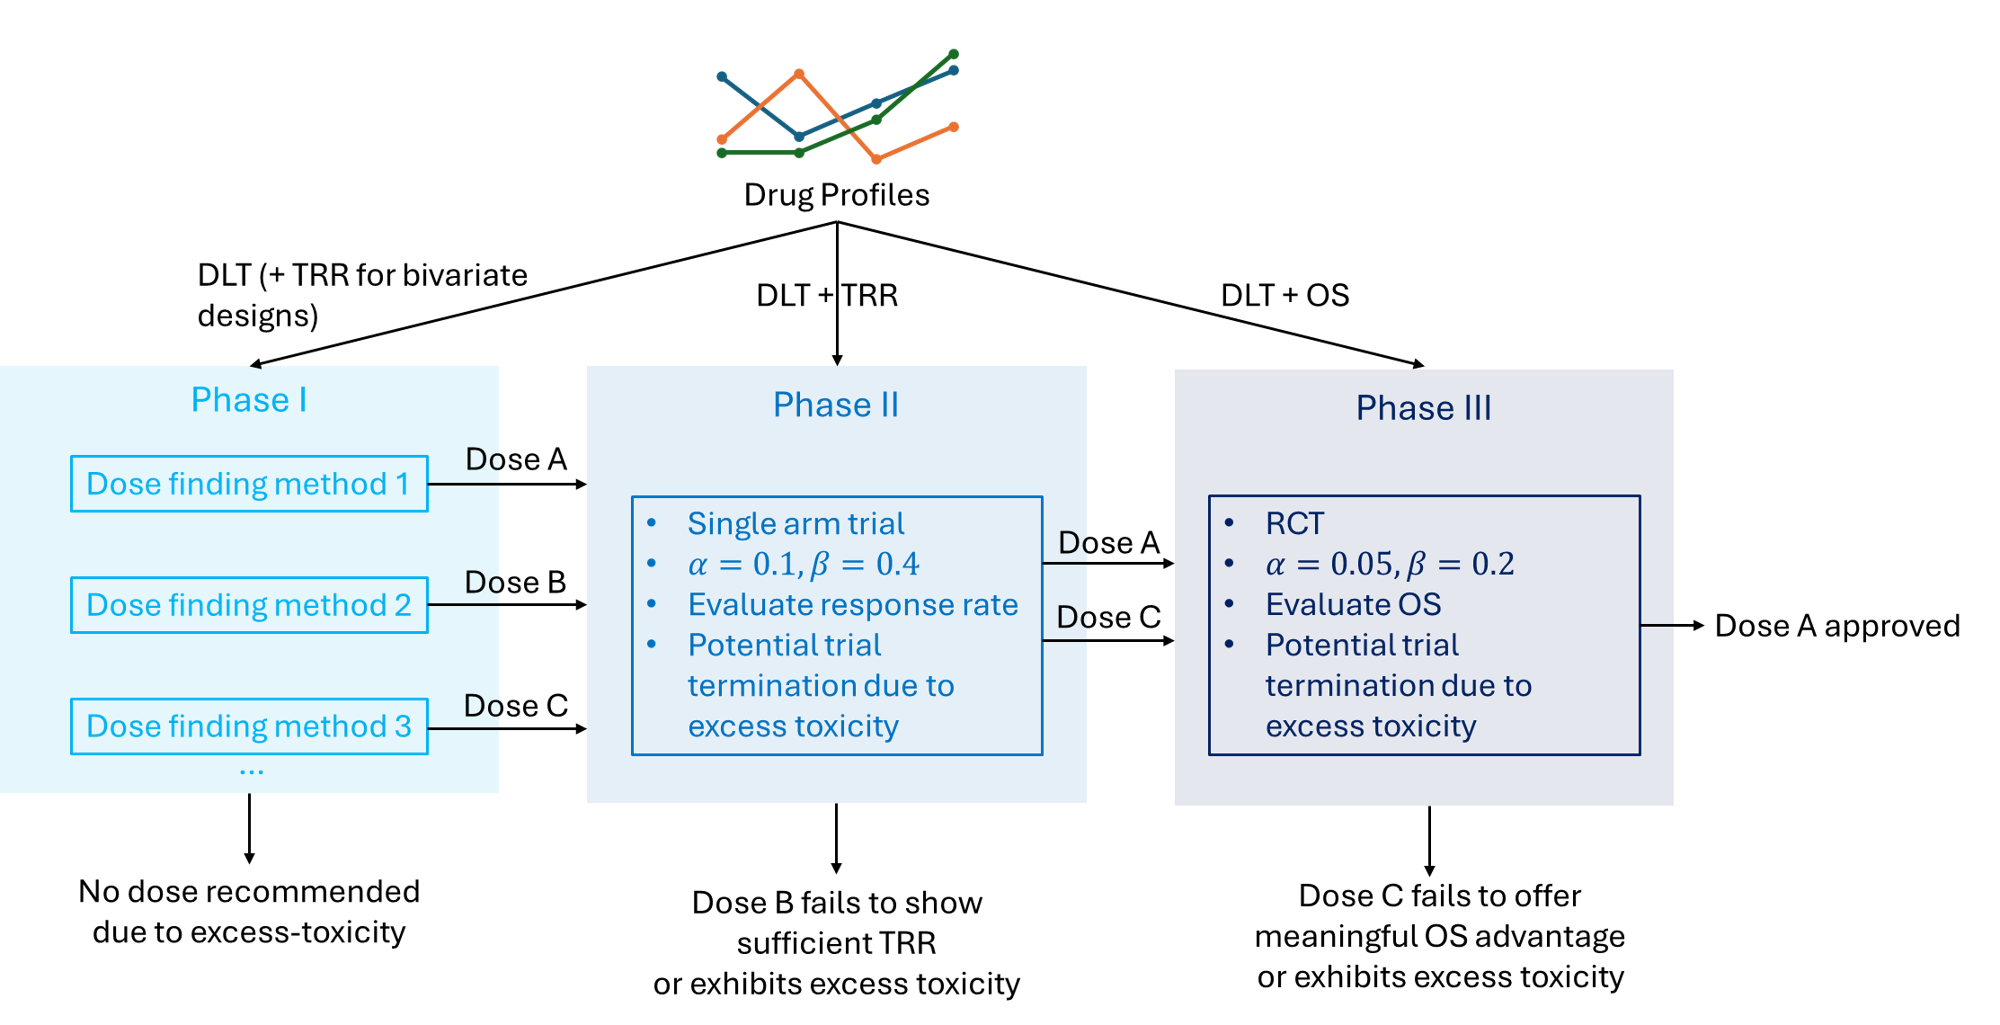
\includegraphics[width=0.95\textwidth]{plots/simulation_framework.png}
\caption{Overall workflow of the simulation. DLT: dose-limiting toxicity. TRR: tumor response rate. OS: overall survival. RCT: randomized controlled trial.}
\label{simulation-framework}
\end{figure}

\subsection{Drug profiles}
A drug profile is defined by three key relationships: the dose-toxicity curve describes the probability of experiencing a dose-limiting toxicity (DLT) at each dose level; the dose-response curve describes the tumor response rate (TRR) at each dose level; and the dose-survival curve describes the median overall survival (OS) at each dose level, assuming an exponential survival distribution. 

To evaluate the robustness of dose-finding methods across different therapeutic scenarios, we considered two representative families of drug profiles. In chemotherapy-like profiles, the dose-response and dose-survival curves increase monotonically with dose level, reflecting the classical oncological assumption that higher doses up to the tolerance threshold are generally associated with higher efficacy. We constructed two chemotherapy-like profiles, one with a flat efficacy increase and the other with a steep increase around the MTD of dose 5 (Figure \ref{drug-profile}). In contrast, in immunotherapy-like profiles, the dose-response and dose-survival curves plateau before reaching the MTD. Therefore, the optimal biological dose (OBD) is lower than the MTD, reflecting diminishing gains in efficacy at higher dose levels despite acceptable toxicity \parencite{patil_low_2019}. We constructed two immunotherapy-like profiles, an early plateau with OBD being dose 3 and a late plateau with OBD being dose 4 (Figure \ref{drug-profile}). The specific parameterization of each drug profile is detailed in the Appendix.

\begin{figure}[ht]
    \centering
    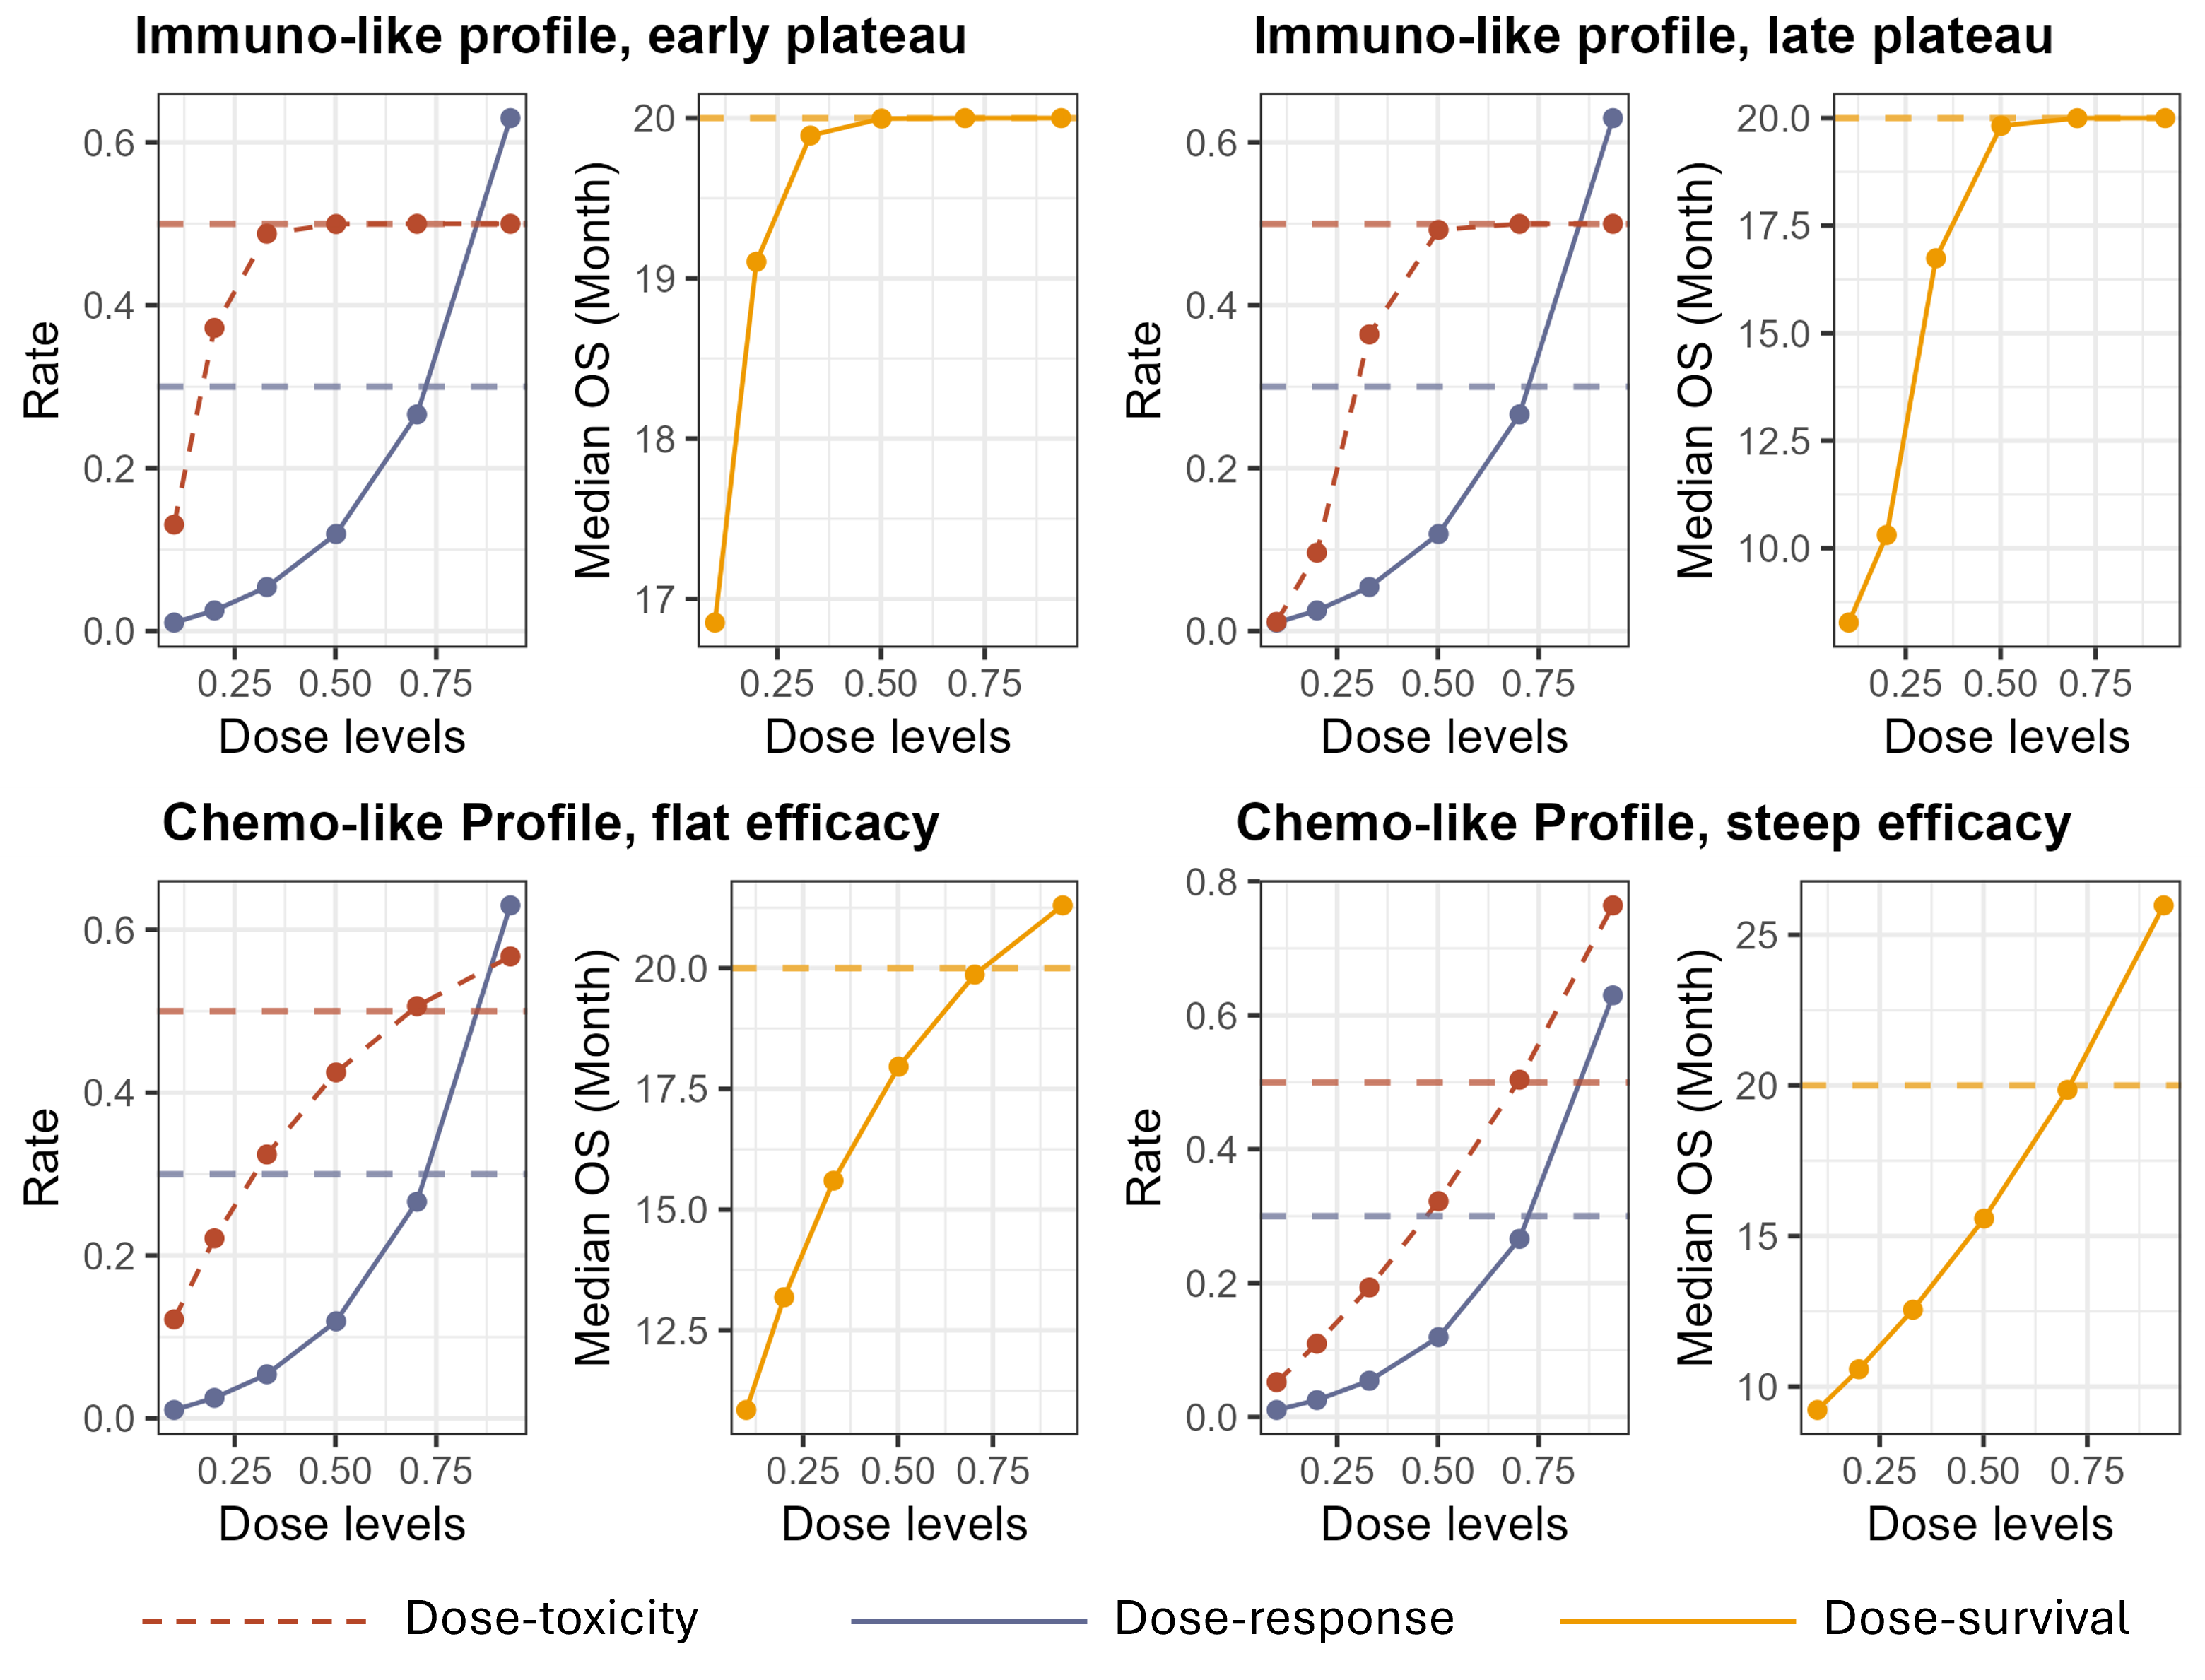
\includegraphics[width=0.9\textwidth]{plots/drug_profiles.png}
    \caption{Dose-toxicity, dose-response, and dose-survival curves for the two chemotherapy-like and two immunotherapy-like drug profiles. The vertical dashed lines indicate the target DLT of $30\%$ for Phase I univariate designs; target TRR of $50\%$ for Phase II designs; target median OS of 20 months for Phase III designs.}
    \label{drug-profile}
\end{figure}

\subsection{Phase I dose-finding methods}
\textcite{clertant2022early} classifies dose-finding methods into three general categories, from which we selected representative methods for comparison (Table \ref{phase1-methods}). 3+3 is the most widely used design in practice and serves as a benchmark for comparison. Due to its stochastic nature, neither the sample size nor the target DLT rate can be explicitly defined, but its empirical target DLT is typically around $16\%$ to $27\%$ based on simulation studies \parencite{chiuzan_3_2024}. BOIN retains the simplicity of rule-based designs while improving statistical efficiency. It compares the observed DLT rate at the current dose with pre-specified escalation and de-escalation boundaries derived from a beta-binomial framework. During dose escalation, doses with posterior probability greater than 0.95 of exceeding the target toxicity were considered inadmissible. At the end of the trial, isotonic regression is applied to all accumulated data to select the MTD \parencite{BOIN}. CRM is a model-based design that continuously updates a parametric dose-toxicity model using all available data. Implementation requires specification of a prior skeleton for the dose-toxicity relationship and an initial prior estimate of the MTD \parencite{CRM}. A known limitation of CRM is its tendency to allocate patients to overly toxic doses. Although alternative designs such as escalation with overdose control (EWOC) have been proposed to tackle this issue, they often involve different model parameterizations and additional tuning parameters \parencite{EWOC}. To align designs compared in our simulation framework, we implemented an overdose control rule similar to that used by BOIN, whereby doses with high posterior probability of exceeding the target DLT rate are excluded from escalation. For both BOIN and CRM, the target DLT rate was set to $30\%$ and sample size to 30 subjects, reflecting common practice in oncology Phase I trials \parencite{li_phase_2024}. 

In addition to these univariate designs, which rely solely on toxicity outcomes, we also considered bivariate designs that jointly incorporate toxicity and efficacy data to guide dose selection and identify the OBD. If the underlying drug profile has an efficacy plateau before the MTD, bivariate designs are expected to outperform univariate designs by trading off toxicity with efficacy and better targeting the OBD. But there are also potential limitations of bivariate designs, such as increased model complexity and estimation uncertainty in small sample sizes, which may compromise their performance.

The BOIN12 design extends BOIN by introducing utilities for the four possible combinations of DLT (yes/no) and tumor response (yes/no) outcomes. A common parametrization fixes utility $u_1$ for (No Toxicity, Response) at 100 and utility $u_4$ for (Toxicity, No Response) at 0, and imposes a constraint that the utility $u_2$ for (No Toxicity, No Response) and utility $u_3$ for (Toxicity, Response) sum up to 100 \parencite{BOIN12}.

The EffTox design extends CRM by jointly modeling dose-toxicity and dose-response relationships using parametric models \parencite{EffTox}. It incorporates the toxicity-efficacy trade-off through a utility contour plot defined by three anchor points (pairs of DLT and response rates), which determine the neutral utility line \parencite{EffTox_hyperparameters}. Doses that lie closer to the right-bottom corner (100\% TRR and 0\% DLT rate) of the contour plots are assigned with higher utility.

For bivariate designs, we additionally included futility stopping rules alongside toxicity control to avoid selecting subtherapeutic doses. Details of utility elicitation and admissibility criteria are summarized in Table \ref{phase1-methods}.

\begin{table}[htbp]
\centering
\caption{Summary of Phase I dose-finding designs considered in the study}
\label{phase1-methods}
\begin{tabularx}{\textwidth}{
 ll
  >{\hsize=0.8\hsize}X
  >{\hsize=1.1\hsize}X
  >{\hsize=1.1\hsize}X
}
\toprule
Method & Design class & Endpoint & Key tuning parameters$^\dagger$ & Admissible criteria$^\S$ \\
\midrule

\multicolumn{5}{l}{\textbf{Univariate designs}} \\

3+3 & Rule-based & DLT & N/A &
Terminate the trial if the first dose indicates de-escalation \\

BOIN & Model-assisted & DLT &
\makecell[l]{Cohort size = 3 \\ Target DLT = 30\%} &
Terminate if the first dose indicates de-escalation; doses with $\ge 0.95$ posterior probability of DLT $>$ target are inadmissible \\

CRM & Model-based & DLT &
\makecell[l]{Cohort size = 1 \\ Target DLT = 30\%}  &
Terminate if the first dose indicates de-escalation; doses with $\ge 0.95$ posterior probability of DLT $>$ target are inadmissible \\

\midrule
\multicolumn{5}{l}{\textbf{Bivariate designs}} \\

BOIN12 & Model-assisted & DLT + tumor response &
Toxicity upper limit $\phi_T=0.35$; Efficacy lower limit $\phi_E=0.5$; Utility table
$u_{1(\text{no tox, eff})}=100, u_{2(\text{no tox, no eff})}=40, u_{3(\text{tox, eff})}=60, u_{4(\text{tox, no eff})}=0$ &
Terminate if the first dose indicates de-escalation; doses with $\ge 0.95$ posterior probability of DLT $\ge \phi_T$ are inadmissible; doses with $\le 0.9$ posterior probability of TRR $\le \phi_E$ are inadmissible \\

EffTox & Model-based & DLT + tumor response &
Toxicity upper limit $\pi_T^*=0.3$: Efficacy lower limit $\pi_E^*=0.5$; 
Utility contour $\pi_1^*=(0.4,0)$, $\pi_2^*=(1,0.7)$, $\pi_3^*=(0.65,0.25)$; 
Prior effective sample sizes ESS$_T$ = ESS$_E$ = 1 &
Terminate if the first dose indicates de-escalation; doses with $\ge 0.95$ posterior probability of DLT $\ge \pi_T^*$ are inadmissible; doses with $\le 0.95$ posterior probability of TRR $\le \pi_E^*$ are inadmissible \\
\bottomrule
\end{tabularx}
\end{table}

\subsection{Phase II and III designs}
Standard designs were implemented in Phase II and III to isolate the effect of dose selection in Phase I (Table \ref{phase23-designs}). In Phase II, a Simon two-stage minimax design was used to evaluate the TRR of the selected RP2D \parencite{simon2stage}. The type I error was controlled at 10\% (two-sided) and the power was targeted to be 80\%. We assumed a TRR of 35\% for the standard-of-care and a target TRR of 50\% for the new drug. A total of 49 subjects was planned, with 31 subjects enrolled in the first stage. The trial continues to the second stage only if more than 10 subjects achieve a tumor response in the first stage. At the end of the trial, efficacy is declared if more than 21 subjects demonstrate tumor response. In Phase III, a two-arm randomized controlled trial (RCT) was used to compare the OS of the selected RP2D against the standard-of-care. The type I error was controlled at 5\% (two-sided) and the power was targeted to be 80\%. We assumed the OS of the standard-of-care followed an exponential distribution with a median OS of 14 months, both for the sample size calculation and for data generation, and the target median OS benefit from the new drug was 6 months. The maximum follow-up time was set to 60 months, with an expected accrual duration of 12 months. A total of 218 subjects was planned, with 109 subjects in each arm.

For both Phase II and III, we considered excess toxicity control rules to represent the safety monitoring that occurs in practice. In real life, safety monitoring of clinical trials is complicated and involves joint discussion and decision-making from the Data Safety Monitoring Board, which is hard to mimic exactly in simulation. We implemented a trial termination rule if the accumulating DLT rate of the treatment arm during the trial exceeds the toxicity suspension threshold (Table \ref{phase23-designs}), with an observation window of 20 patients for Phase II and 30 patients for Phase III. Though being much simplified, this effectively represents different extents of toxicity tolerance in the drug development process, with smaller thresholds reflecting more conservative safety monitoring practices.  

\begin{table}[htbp]
\centering
\caption{Summary of Phase II and III designs used in the study}
\label{phase23-designs}
\begin{tabularx}{\textwidth}{
 l
  >{\hsize=0.9\hsize}X
  >{\hsize=1.1\hsize}X
  >{\hsize=0.9\hsize}X
  >{\hsize=1.1\hsize}X
}
\toprule
Trial Phase & Endpoint & Design & Sample size & Toxicity suspension threshold \\
\midrule
Phase II & Tumor response (yes/no) & \makecell[lt]{Simon two-stage\\design; \\ $\alpha=0.1$ two-sided; \\ $\beta=0.2$} & \makecell[lt]{Stage 1 n=31;\\ Stage 2 n = 18} & 45\% DLT; 40\% DLT; 35\% DLT; 30\% DLT \\
Phase III & Overall survival (months) & \makecell[lt]{1:1 RCT; \\ $\alpha=0.05$ two-sided; \\ $\beta=0.2$} & 109 per arm & 45\% DLT; 40\% DLT; 35\% DLT; 30\% DLT \\
\bottomrule
\end{tabularx}
\end{table}
\subsection{Sensitivity analysis of bivariate designs}
The performance of bivariate designs depends on the specification of utility parameters, which are often elicited from clinical experts and may be subject to uncertainty. We therefore conducted sensitivity analyses to evaluate how different utility specifications impact the performance of BOIN12 and EffTox.

For BOIN12, we varied $u_2$ from 10 to 90, with larger values of $u_2$ placing greater emphasis on avoiding toxicity relative to achieving response. For EffTox, we investigated a series of eight contour plots, two of flat linear shape (FL1, FL2), two of steep linear shape (SL1, SL2), two of flat concave shape (FC1, FC2) and two of steep concave shape (SC1, SC2) (Figure \ref{plot-EffTox-Contour}).

\subsection{Evaluation metrics}
For Phase I-specific operating characteristics, we evaluate the probability of correctly selecting the MTD (for chemotherapy-like profiles) or OBD (for immunotherapy-like profiles); the number of patients treated at dose 6, which is an overly toxic dose with 63\% DLT rate; the number of patients treated at subtherapeutic doses, with subtherapeutic doses defined as giving TRR lower than 35\% assumed for the standard-of-care or giving OS lower than that of the standard-of-care (14 months).

For the entire drug development process, we evaluate the probability of overall success (PoS), defined as the proportion of simulated Phase I-III trial sequences that are not terminated for toxicity and declare statistical significance at the end of the Phase III.
\subsection{Imatinib example}
To illustrate the proposed simulation framework, we redesigned the clinical development process of Imatinib in patients with advanced gastrointestinal stromal tumour (GIST). The challenge in creating real-world drug profiles is that in later phases of drug development, only one or two doses have been investigated. Therefore, there is limited information on response rates and survival times of doses that were not carried on to Phase II and Phase III. However, the PK/PD data from the Phase II trial of Imatinib were reported \parencite{demetri2009imatinib}. Due to heterogeneity in individual absorption/clearance rate, patient cohorts that receive that same dose will still have different serum concentrations of the drug. As a result, we can use drug exposure as a surrogate for drug dose. 

The data generation was divided into two steps. We first generated the exposure data for the patient cohort receiving different doses based on their relevant pharmacological characteristics (Figure \ref{Dist-Imatinib-Cmin}). Then we mapped the simulated exposure to clinical outcomes via the constructed exposure-toxicity, exposure-response, exposure-survival curves derived from clinical reports \parencite{demetri2009imatinib}. Because of the variation in Imatinib exposure, the resulting dose-toxicity, dose-response and dose-survival curves are stochastic rather than fixed. Figure \ref{Imatinib-dose-profile} illustrates 100 simulated Imatinib profiles. Details of the data generation process are described in the Appendix. 

We then applied the simulation framework to evaluate the PoS under different Phase I dose-finding designs and late-phase toxicity control rules. The Phase II and Phase III designs were reconstructed based on the actual designs used in the clinical development of Imatinib. The original Phase II trial of Imatinib was an RCT comparing the 400 mg dose to the 600 mg dose \parencite{demetri2002efficacy}. Its statistical plan specified that recruitment would continue only if at least 3 of 18 treated patients in each arm achieved a response, with a target TRR of 30\%. We adapted this design to a single-arm Simon two-stage design with a total of 37 patients and 18 patients in the first stage. The original Phase III trial of Imatinib was an RCT comparing the 400 mg dose to the 800 mg dose \parencite{blanke2008phase}. A median progression-free survival (PFS) of 18 months was assumed for the lower dose and a hazard ratio for survival of 1.4 was expected for the high dose. The target power was 92\%. The accural was estimated to take 2 years, plus an extra year for follow-up. We calculated the sample size accordingly and we ended up with 310 patients per arm. The toxicity suspension thresholds were set to be the same as those used in the main analysis for comparability.

\begin{figure}[ht]
    \centering
    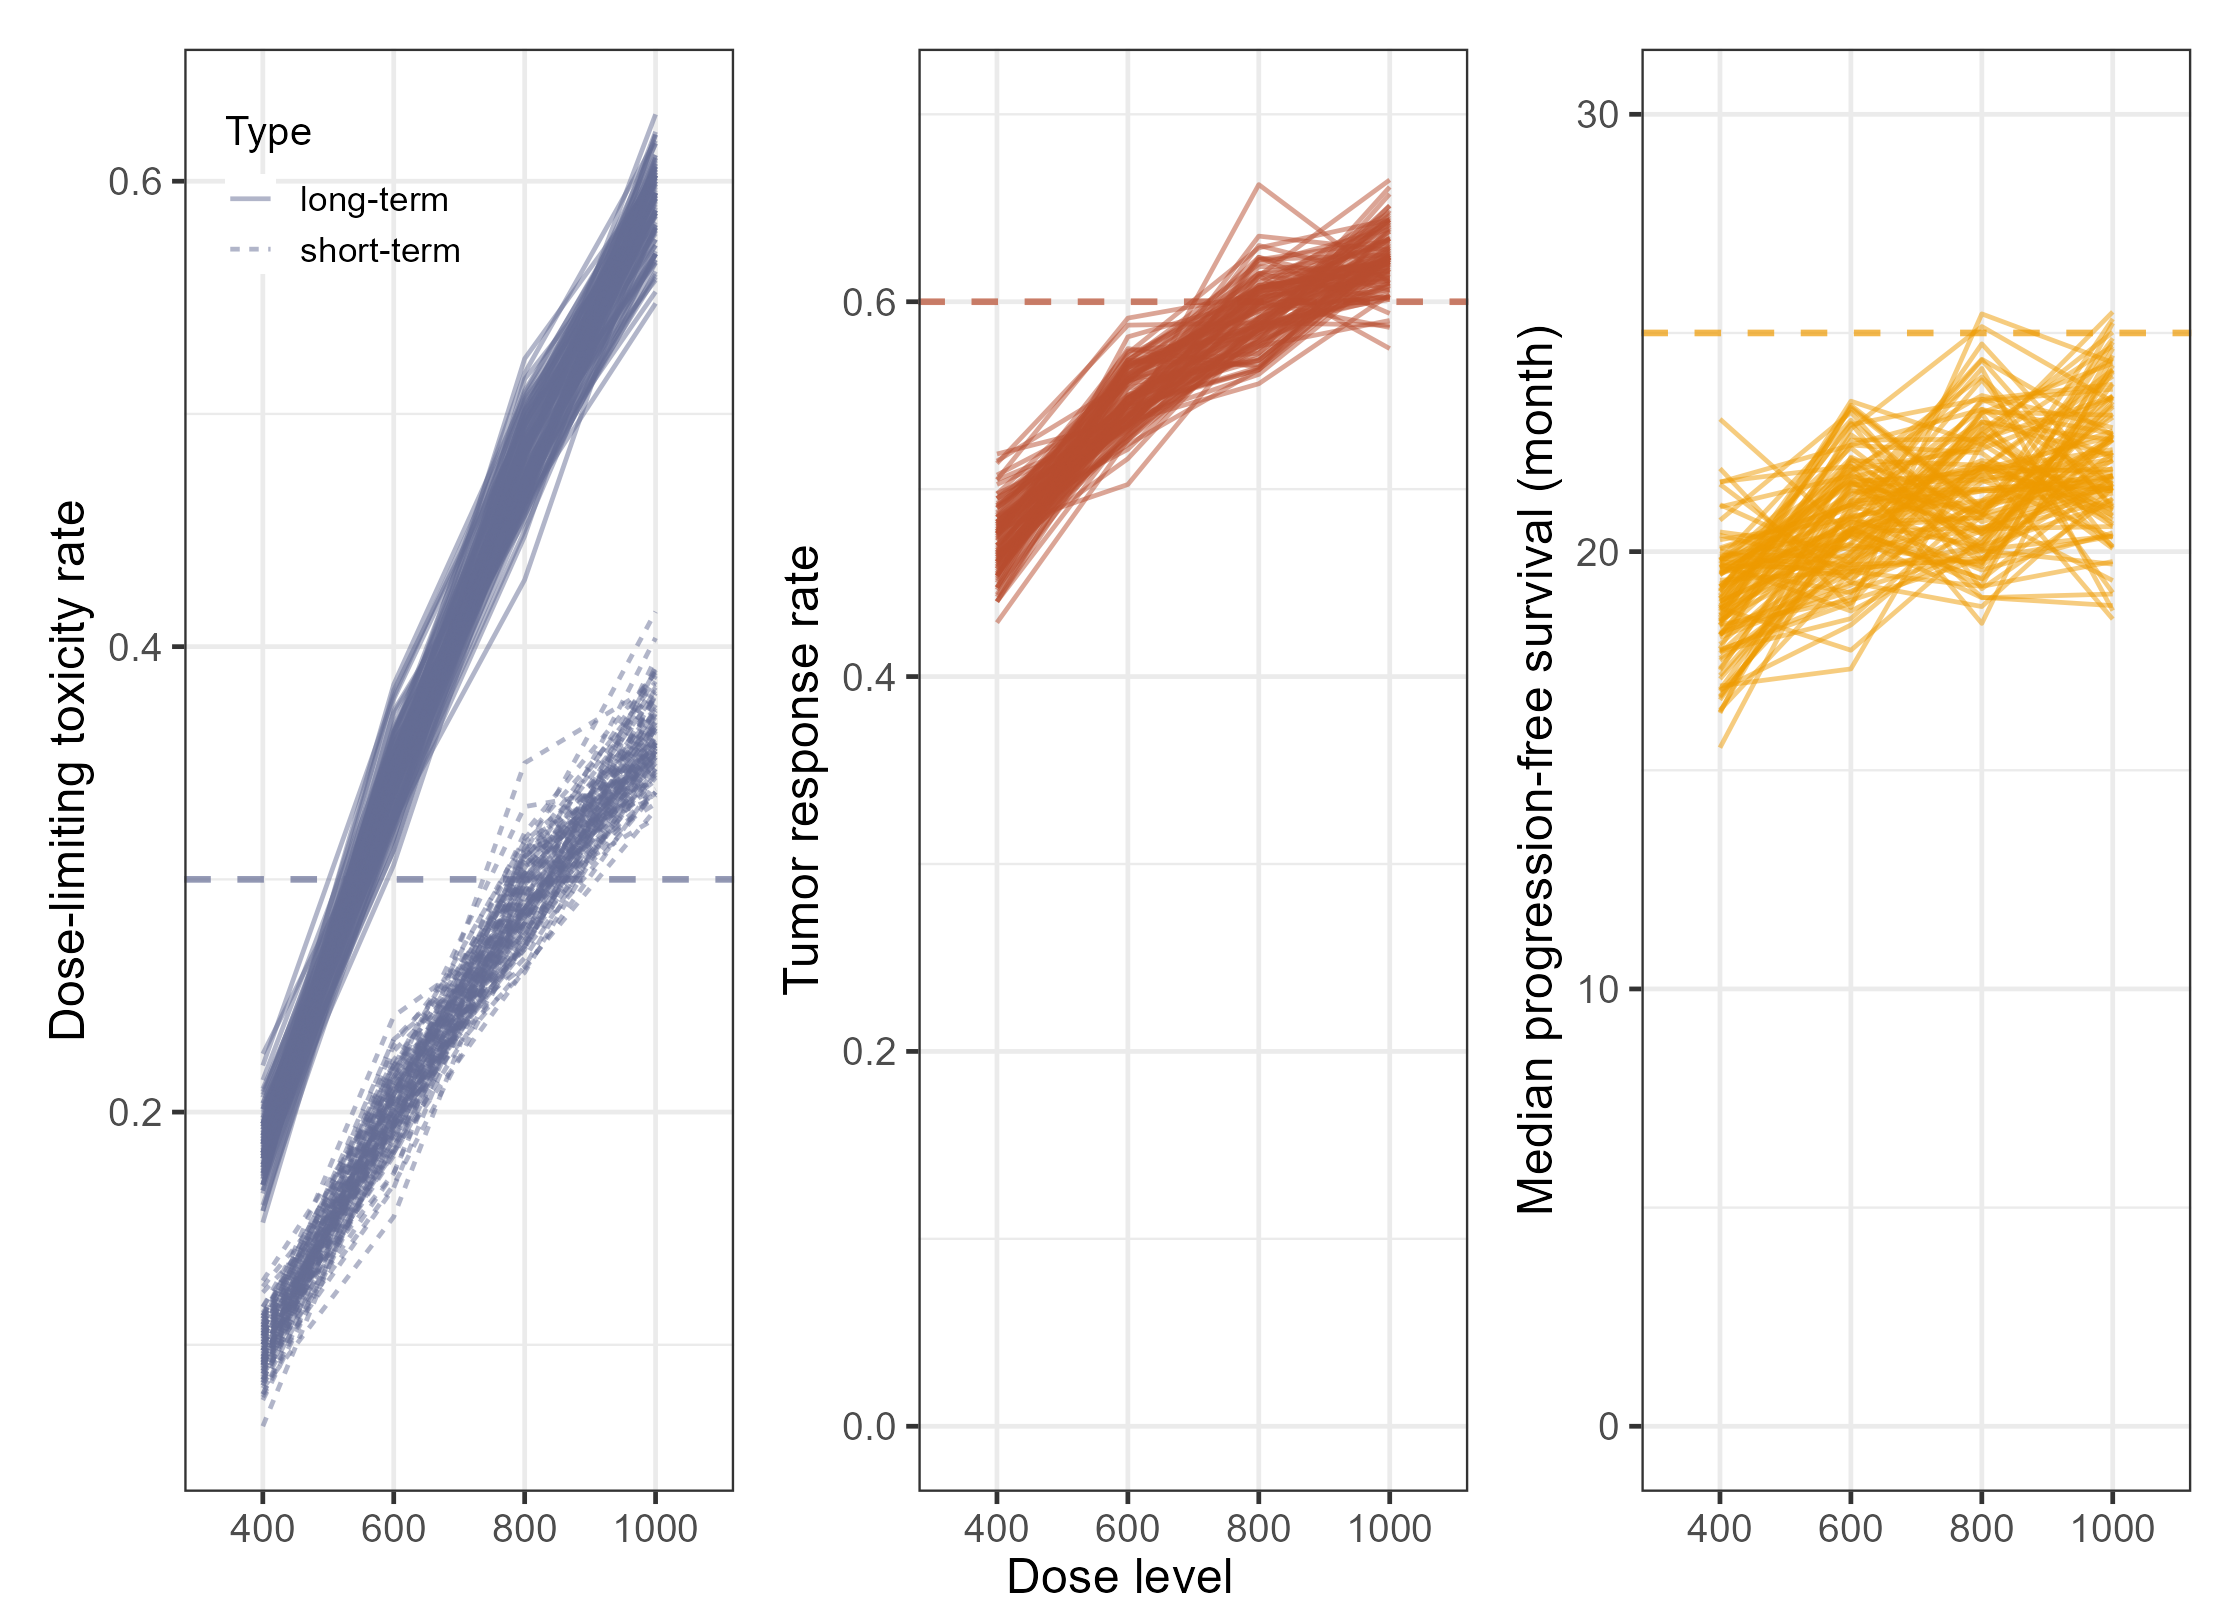
\includegraphics[width=0.8\textwidth]{plots/Imatinib_dose_profile.png}
    \caption{Dose-DLT rate, dose-TRR, and dose-median PFS curves for 100 simulated Imatinib profiles. The vertical dashed lines indicate the target DLT of $30\%$ in the Phase I trial; target TRR of $30\%$ in the Phase II trial; target median PFS of 18 months in the Phase III trial.}
    \label{Imatinib-dose-profile}
\end{figure}
\section{Results}
\subsection{Phase I-specific operating characteristics}
The probability of selecting each dose as the RP2D is shown in Figure \ref{phase1-dose-selection}. For univariate designs that utilize only toxicity data to identify the MTD, the dose selection across four drug profiles is the same as they share the same dose-toxicity curve, with dose 5 being the MTD under a target DLT of 30\%. The 3+3 design gives rather conservative dose selection, with 33\% probability of selecting the MTD, 46\% selecting one dose below the MTD, and 15\% selecting two doses below the MTD. In contrast, BOIN and CRM perform similarly and both can identify the MTD at a moderately high rate of 69\% and 74\%, respectively. Moreover, either the MTD or one dose below the MTD is selected in around 90\% of the times. CRM has a higher probability of recommending the overly toxic dose 6 (12\%) compared to BOIN (3\%), despite the fact that overdose control has been implemented. 

For bivariate designs that jointly consider toxicity and efficacy data to identify the OBD, the dose selection varies across drug profiles. For chemotherapy-like profiles, bivariate designs are generally less efficient in identifying the MTD compared to their univariate counterparts as the additional efficacy information provides limited benefit under monotonic dose-efficacy relationships while increasing model complexity and estimation uncertainty in small-sample settings. For immunotherapy-like profiles, bivariate designs have decent performance in identifying the OBD: BOIN12 identifies the OBD at a rate of 36\% and 40\% for the early and late plateau profiles, respectively; EffTox identifies the OBD at a rate of 33\% and 45\% for the early and late plateau profiles, respectively. Moreover, in occasions when the true OBD is not selected, BOIN12 tends to recommend one dose lower while EffTox one dose higher. Hence, EffTox exhibits more aggressive dose selection behavior relative BOIN12.

\begin{figure}[htbp]
    \centering
    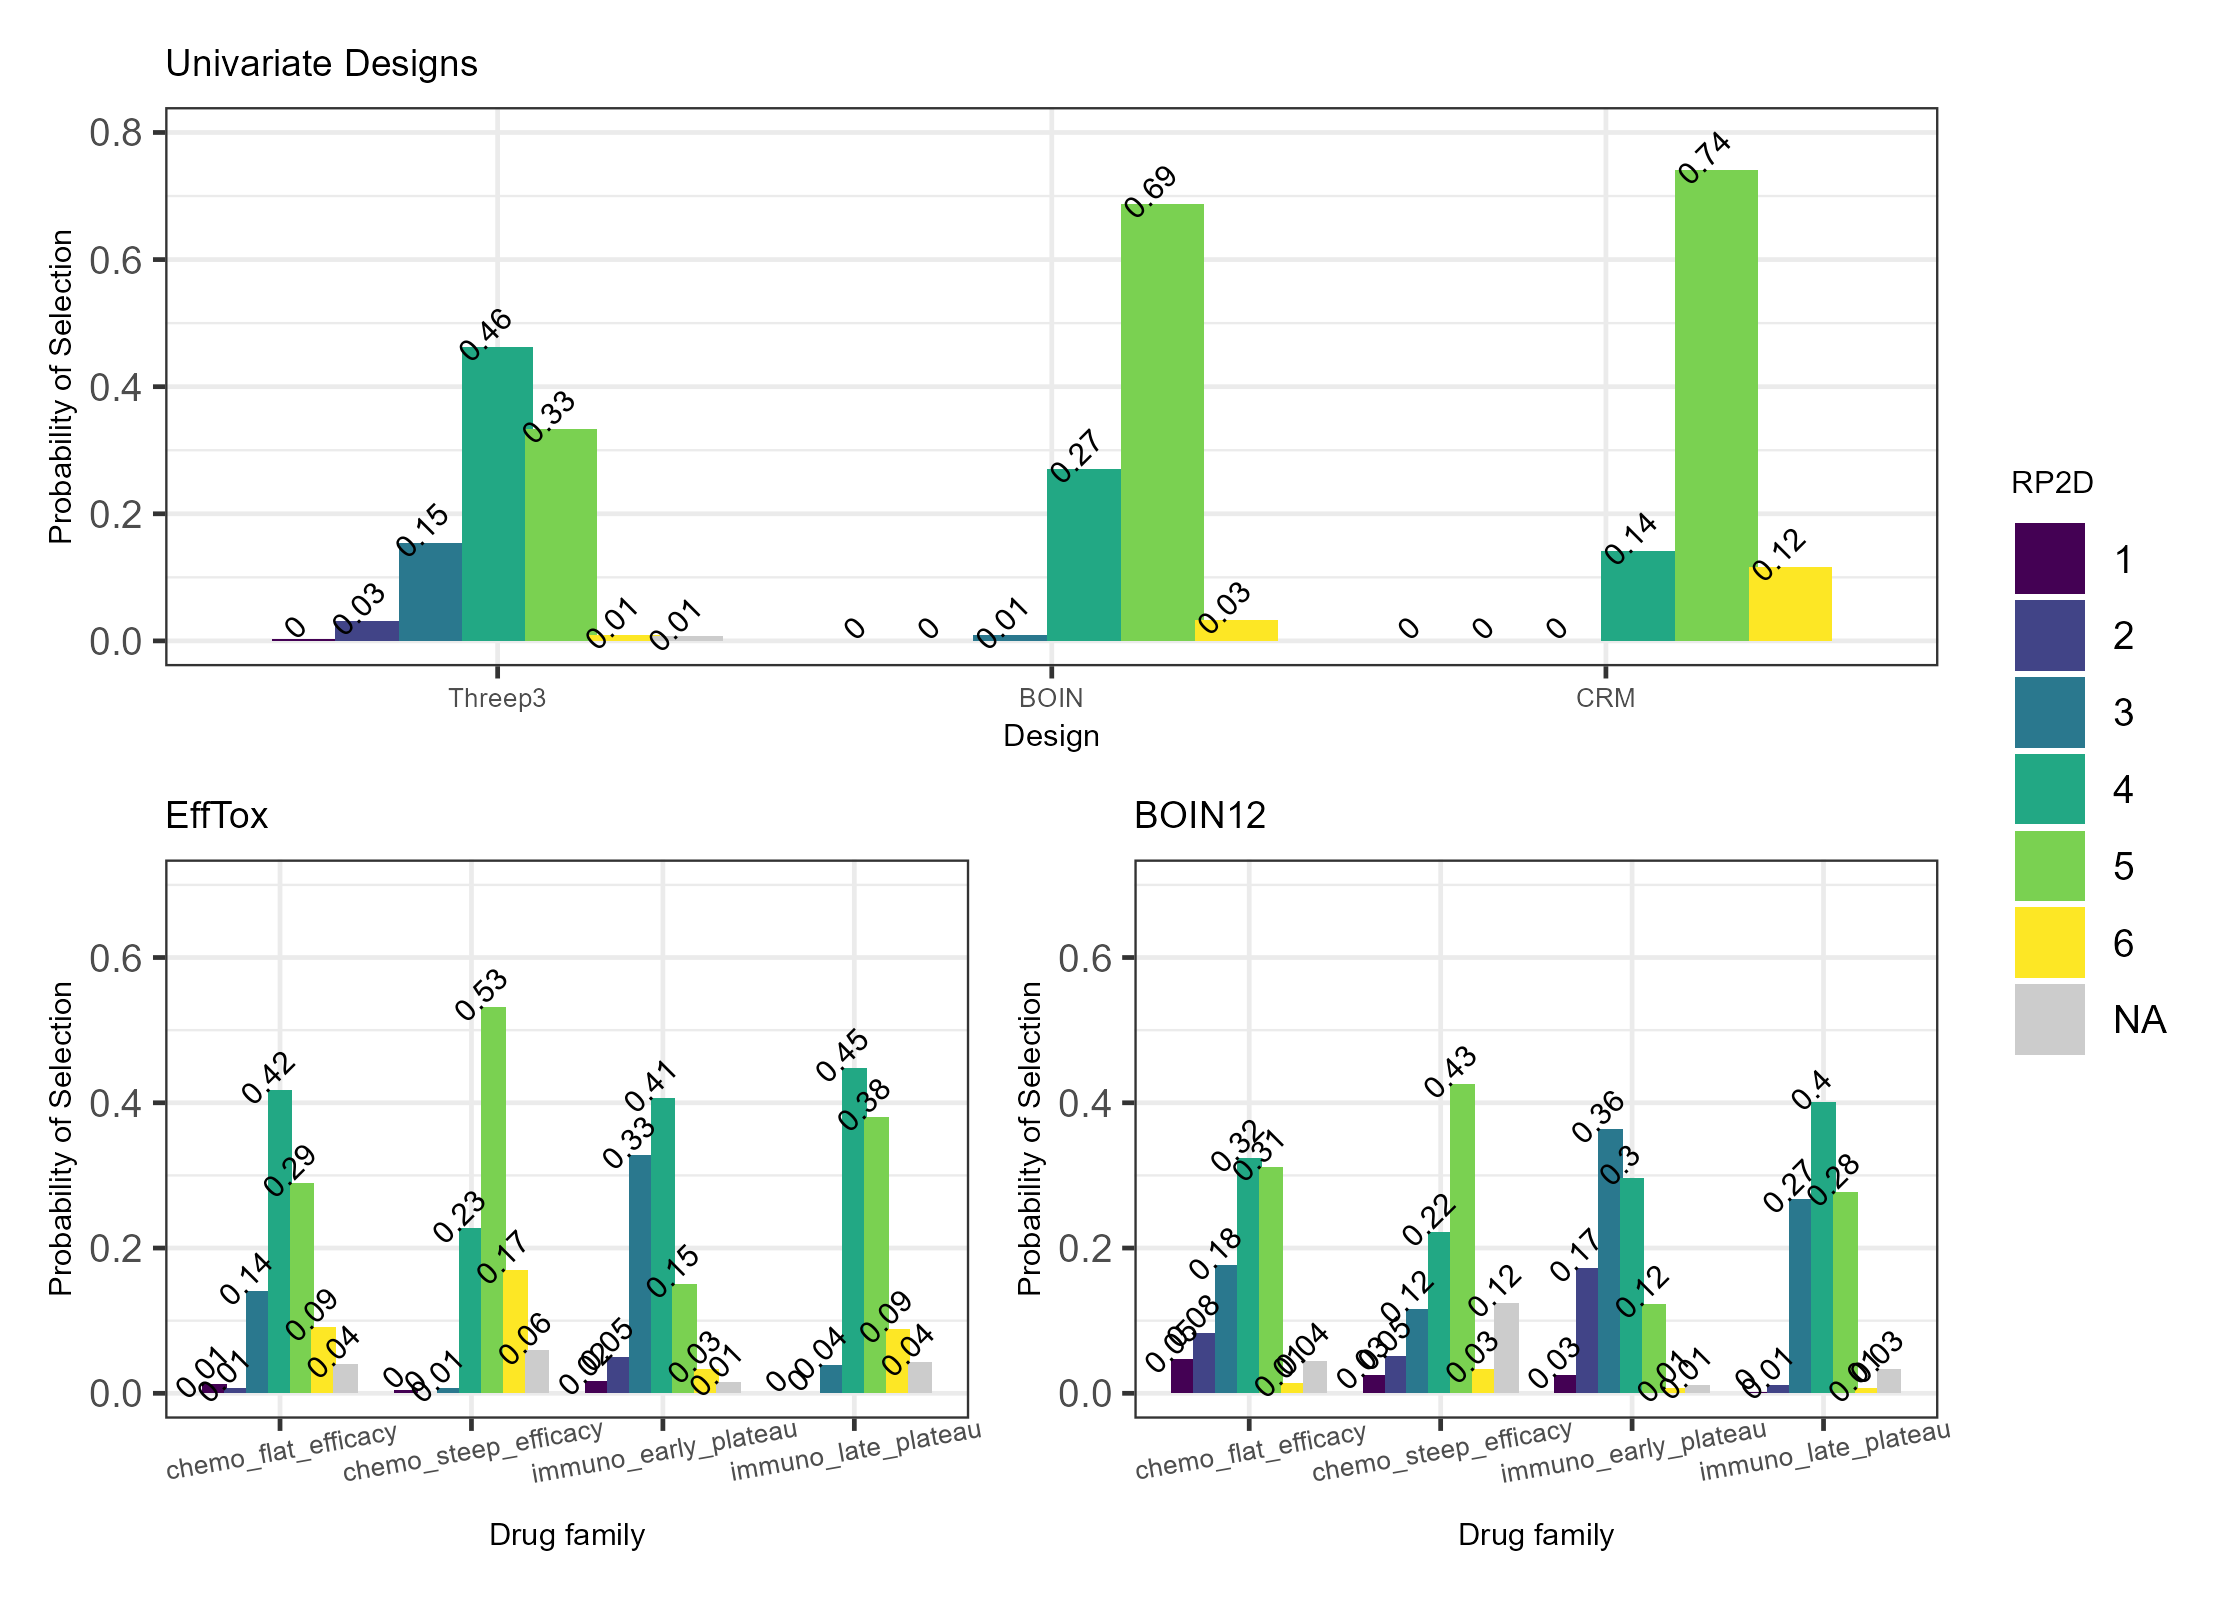
\includegraphics[width=0.98\textwidth]{plots/phase1_dose_selection.png}
    \caption{Probability of selecting each dose as the RP2D across 1000 simulated Phase I trials for univariate designs (top) and bivariate designs (bottom). NA means the Phase I trial is terminated early and no RP2D is selected. For univariate designs and bivariate designs in chemotherapy-like profiles, the target dose is the MTD (dose 5) in green; for bivariate designs in immunotherapy-like profiles, the target dose is the OBD (dose 3 for early plateau and dose 4 for late plateau) in blue.}
    \label{phase1-dose-selection}
\end{figure}

In terms of the dose allocation during the trial, CRM yields a slightly higher proportion of patients being treated at the overly toxic dose 6, but also a much lower proportion of patients being treated at subtherapeutic doses especailly in chemotherapy-like profiles. In immunotherapy-like profiles, the bivariate designs have more desirable patient allocation compared to their univariate counterparts. For example, BOIN12 achieved similar proportion of underdosing and less proportion of overdosing compared to BOIN (Figure \ref{phase1-under-overdose}). 

In summary, when toxicity drives optimal dosing as in chemotherapy-like profiles, incorporating efficacy information does not improve, and may even compromise the MTD selection. For immunotherapy-like profiles where the optimal dose requires a balance between toxicity and efficacy, bivariate designs improve OBD targeting, though it is still more challenging to identify the OBD compared to the MTD in chemotherapy-like profiles. 

\begin{figure}[htbp]
    \centering
    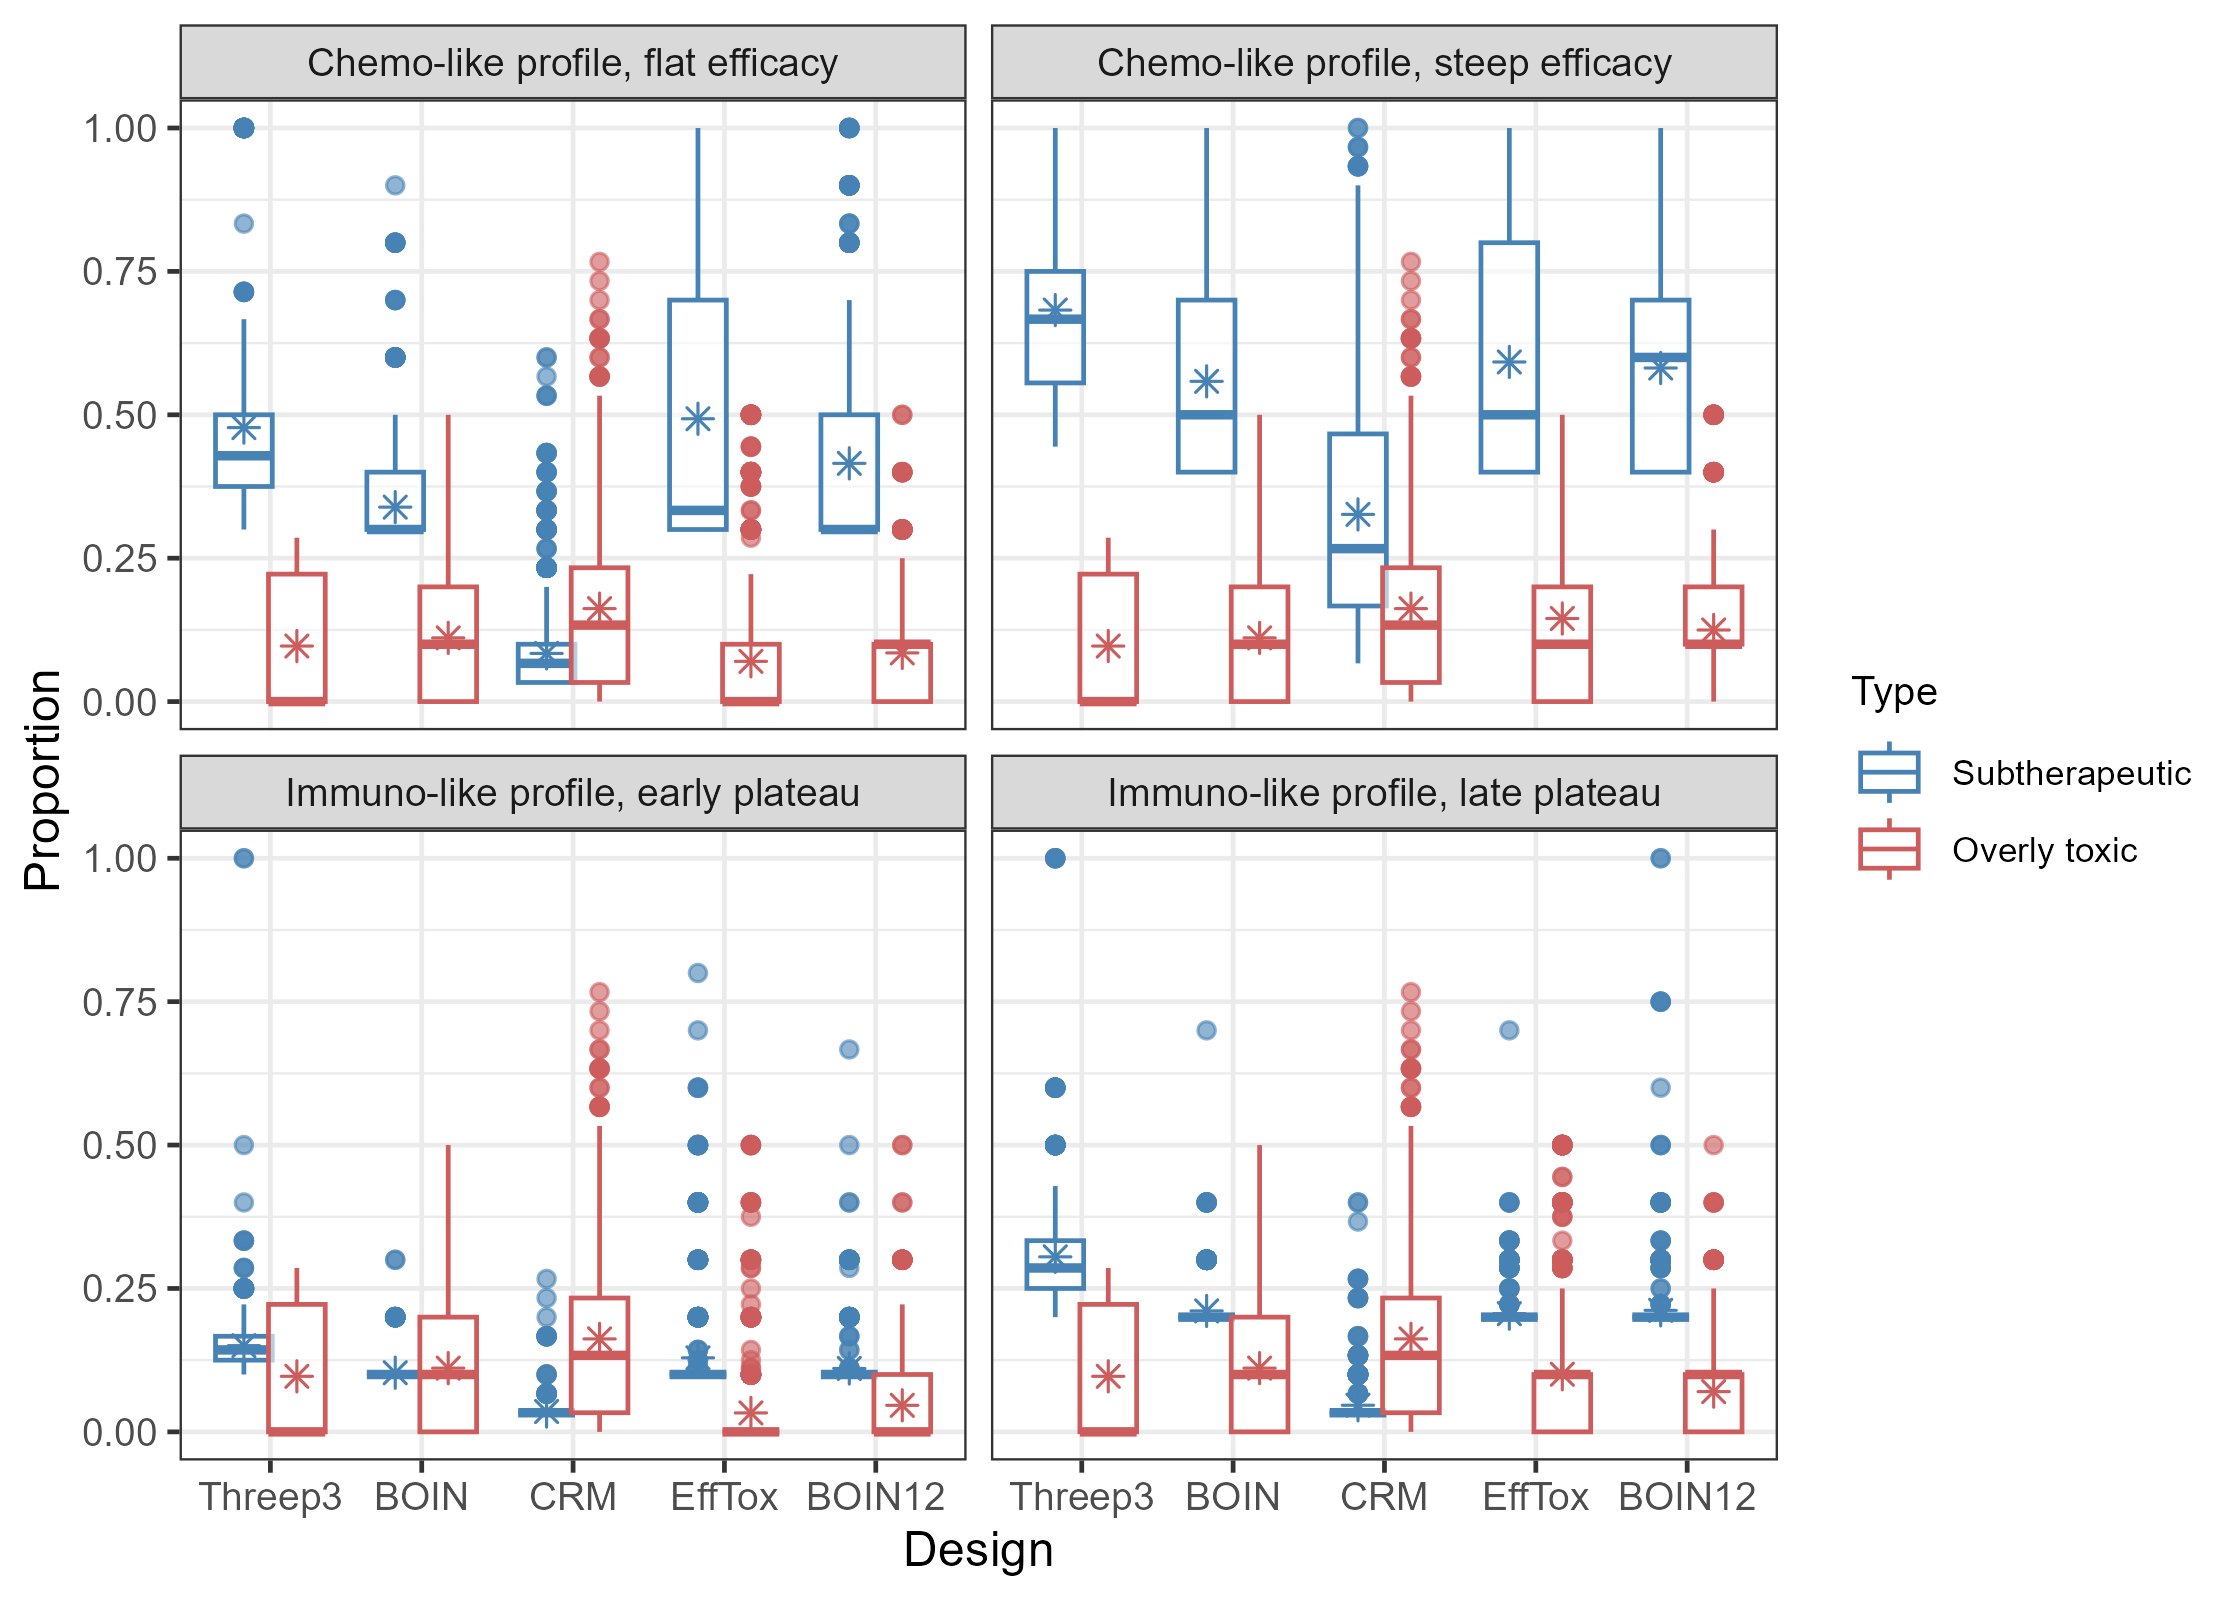
\includegraphics[width=0.95\textwidth]{plots/phase1_under_overdose.png}
    \caption{Distribution of the proportion of patients treated at the overly toxic dose 6 and subtherapeutic doses across 1000 simulated Phase I trials. The star marks the mean value.}
    \label{phase1-under-overdose}
\end{figure}

\subsection{Probability of overall success (PoS)}
For chemotherapy-like profiles, BOIN and CRM outperform 3+3 and give consistently higher PoS (Figure \ref{plot-PoS}). Their advantage over 3+3 is more evident under more liberal toxicity control, whereas the performance gap narrows when toxicity control becomes stricter. In these settings, excessive toxicity is penalized more severely than insufficient efficacy, and the conservative nature of the 3+3 design makes it less likely to trigger trial suspension due to excess toxicity. When a very strict suspension threshold of 30\% DLT is applied, all methods yield low PoS around or below 20\% (Figure \ref{plot-PoS}). There is limited benefit from incorporating efficacy data in Phase I dose-finding procedures. This is expected because, for cytotoxic agents, the MTD is typically a clinically appropriate target. Bivariate designs that balance toxicity and efficacy tend to be more conservative and frequently recommend doses below the MTD, thus leading to lower PoS. 

For immunotherapy-like profiles, bivariate designs give more stable PoS across toxicity control rules (Figure \ref{plot-PoS}): they target OBD properly and lead to fewer trials being suspended due to excess toxicity (Figure \ref{plot-PoTS}). For example, in the early-plateau scenario, the PoS of BOIN12 decreases by 10.1\% (from 50.4\% to 45.3\%) when moving from no toxicity control to the 30\% DLT toxicity suspension threshold, whereas the PoS of BOIN drops by 44.2\% (from 54.8\% to 30.6\%). The location of the efficacy plateau is also an influential factor on PoS. In the setting of an early plateau, accurate MTD selection does not translate into high overall PoS. BOIN and CRM that efficiently target the MTD are penalized in later phases due to unnecessary toxicity and therefore have higher probability of trial suspension due to excessive toxicity (Figure \ref{plot-PoTS}). Under moderately strict toxicity control rules, their PoS even drops below that of 3+3. For the late-plateau profile, methods that target MTD achieve relatively good PoS since the OBD and MTD are close. Bivariate designs outperform BOIN and CRM mainly under relative strict toxicity control where the unnecessary toxicity associated with targeting the MTD instead of the OBD is more strongly penalized. The difference between EffTox and BOIN12 is enlarged compared to the early-plateau case, particularly when the toxicity control rule is more liberal. In this setting, the aggressiveness of EffTox is less penalized and its better OBD targeting leads to higher PoS compared to BOIN12.

The PoS decreases uniformly as the toxicity control in Phase II and Phase III becomes more stringent. This trend reflects increasing failure rate of the drug development process due to unmanageable toxicity. The interaction between aggressive Phase I dose selection strategy and strict downstream toxicity control can have a major impact on the final PoS. For example, using CRM in Phase I together with a 30\% toxicity suspension threshold in Phase II and Phase III leads to more than 60\% of the trials being suspended after Phase I in all drug profiles (Figure \ref{plot-PoTS}). Flat and high PoS curves in Figure \ref{plot-PoS} therefore indicate robust performance in selecting the optimal dose and fewer resources wasted in failed late-phase trials, which is desirable given the uncertainty in how toxicity will be monitored in practice. 

\begin{figure}[htbp]
    \centering
    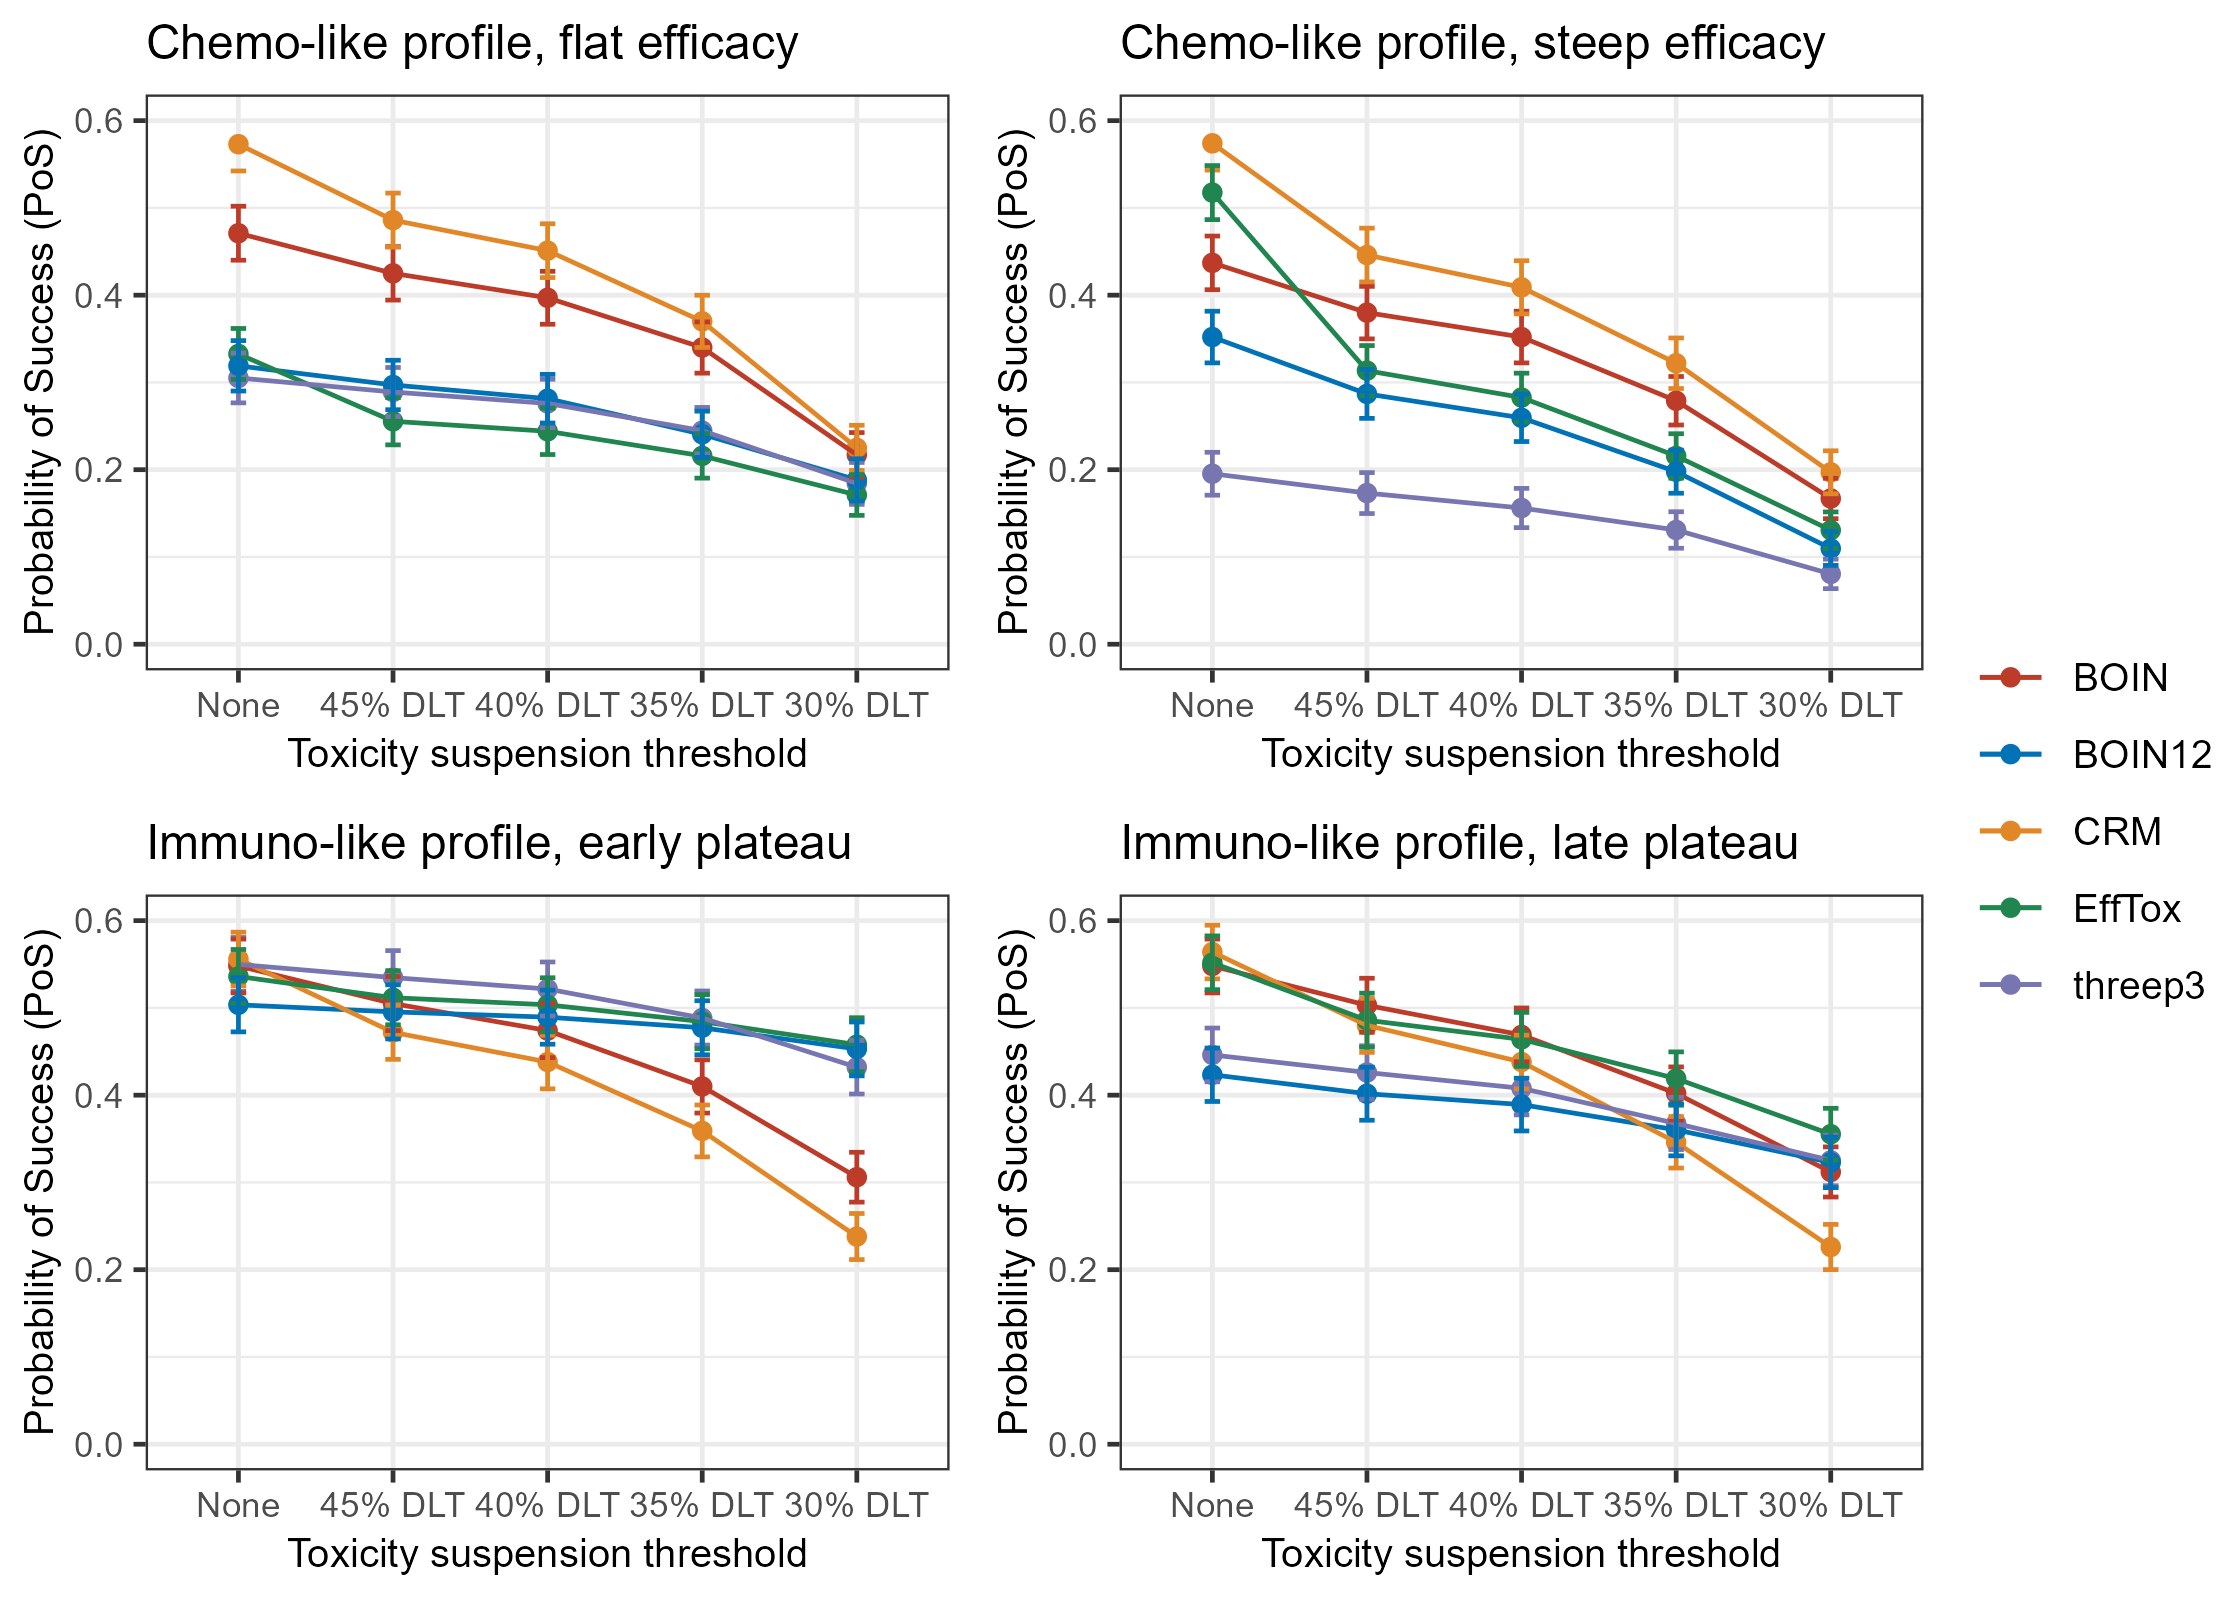
\includegraphics[width=0.95\textwidth]{plots/plot_PoS.png}
    \caption{Probability of overall success (PoS) across different Phase I dose-finding designs and late-phase toxicity control settings for chemotherapy-like and immunotherapy-like drug profiles. The error bars represent 95\% Monte Carlo confidence intervals.}
    \label{plot-PoS}
\end{figure}
\subsection{Sensitivity analysis results}
For BOIN12, as $u_2$, the utility value for outcome combination (No Toxicity, No Response), increases, the design becomes more conservative with increasing probability of selecting one dose below the OBD than one dose above it. But the probability of selecting the OBD is relatively stable across different values of $u_2$ (Figure \ref{plot-sens-BOIN12-RP2D}). Under liberal toxicity control, the PoS shows moderate variation across different values of $u_2$, except in the chemotherapy-like profile with a steep efficacy increase, where the PoS is nearly unchanged. Immuno-agents often show efficacy at doses much lower than the MTD. Hence it makes sense to set $u_2 < u_3$, i.e., $u_2 \lt 50$ to weigh efficacy more than toxicity. For this range of utility specification, the PoS is relatively robust with nearly overlapping curves (Figure \ref{plot-sens-BOIN12-PoS}). 

For EffTox, the shape of the contour plots has a major impact on dose selection. The OBD in immunotherapy-like profiles is better identified with a linear-shaped utility contour while the MTD in chemotherapy-like profiles is better targeted with a concave-shaped utility contour (Figure \ref{plot-sens-EffTox-RP2D}). Thus, the optimal contour shape depends strongly on the underlying drug profile. PoS varies more across contour specifications for EffTox than across utility choices for BOIN12. For immunotherapy-like profiles, PoS differences become more pronounced under stricter toxicity control while for chemotherapy-like profiles, differences across contour shapes diminish as toxicity control becomes stricter. The contour used in the main analysis is well tuned for immunotherapy-like profiles and achieves relatively high PoS among the evaluated shapes (Figure \ref{plot-sens-EffTox-PoS}). 

Overall, BOIN12 demonstrates relatively stable performance across a wide range of utility specifications, with modest changes in dose selection and PoS. In contrast, EffTox is more sensitive to the shape of the utility contour, and its performance depends more strongly on how well the contour aligns with the underlying dose-toxicity/response relationship.

\section{Imatinib example results}
The PoS of Imatinib development is generally higher than the generic drug profiles, which is expected given the large improvement in therapeutic effect of Imatinib compared to standard-of-care. The PoS is close to one under no late phase toxicity control due to its well-powered Phase II and III trials. However, the PoS drops rapidly as the toxicity control becomes more stringent. This decrease reflects the discprepancy between the relatively manageable short-term DLT observed within the first 8 weeks in Phase I and the more severe long-term toxicity profile of Imatinib (Figure \ref{Imatinib-dose-profile}), leading to a higher rate of trial suspension (Figure \ref{plot-Imatinib}). If dose selection were based solely on short-term DLT, the 800 mg dose could be considered the OBD because it provides additional tumor response and PFS benefit while maintaining acceptable short-term toxicity. However, when long-term toxicity is incorporated, lower doses such as 400 mg or 600 mg may arguably be the OBD as they provide a more favorable balance between efficacy and safety. The EffTox design gives the highest PoS across all late-phase toxicity control rules, followed by 3+3, BOIN12, BOIN and CRM (Figure \ref{plot-Imatinib}). 

\begin{figure}[ht]
    \centering
    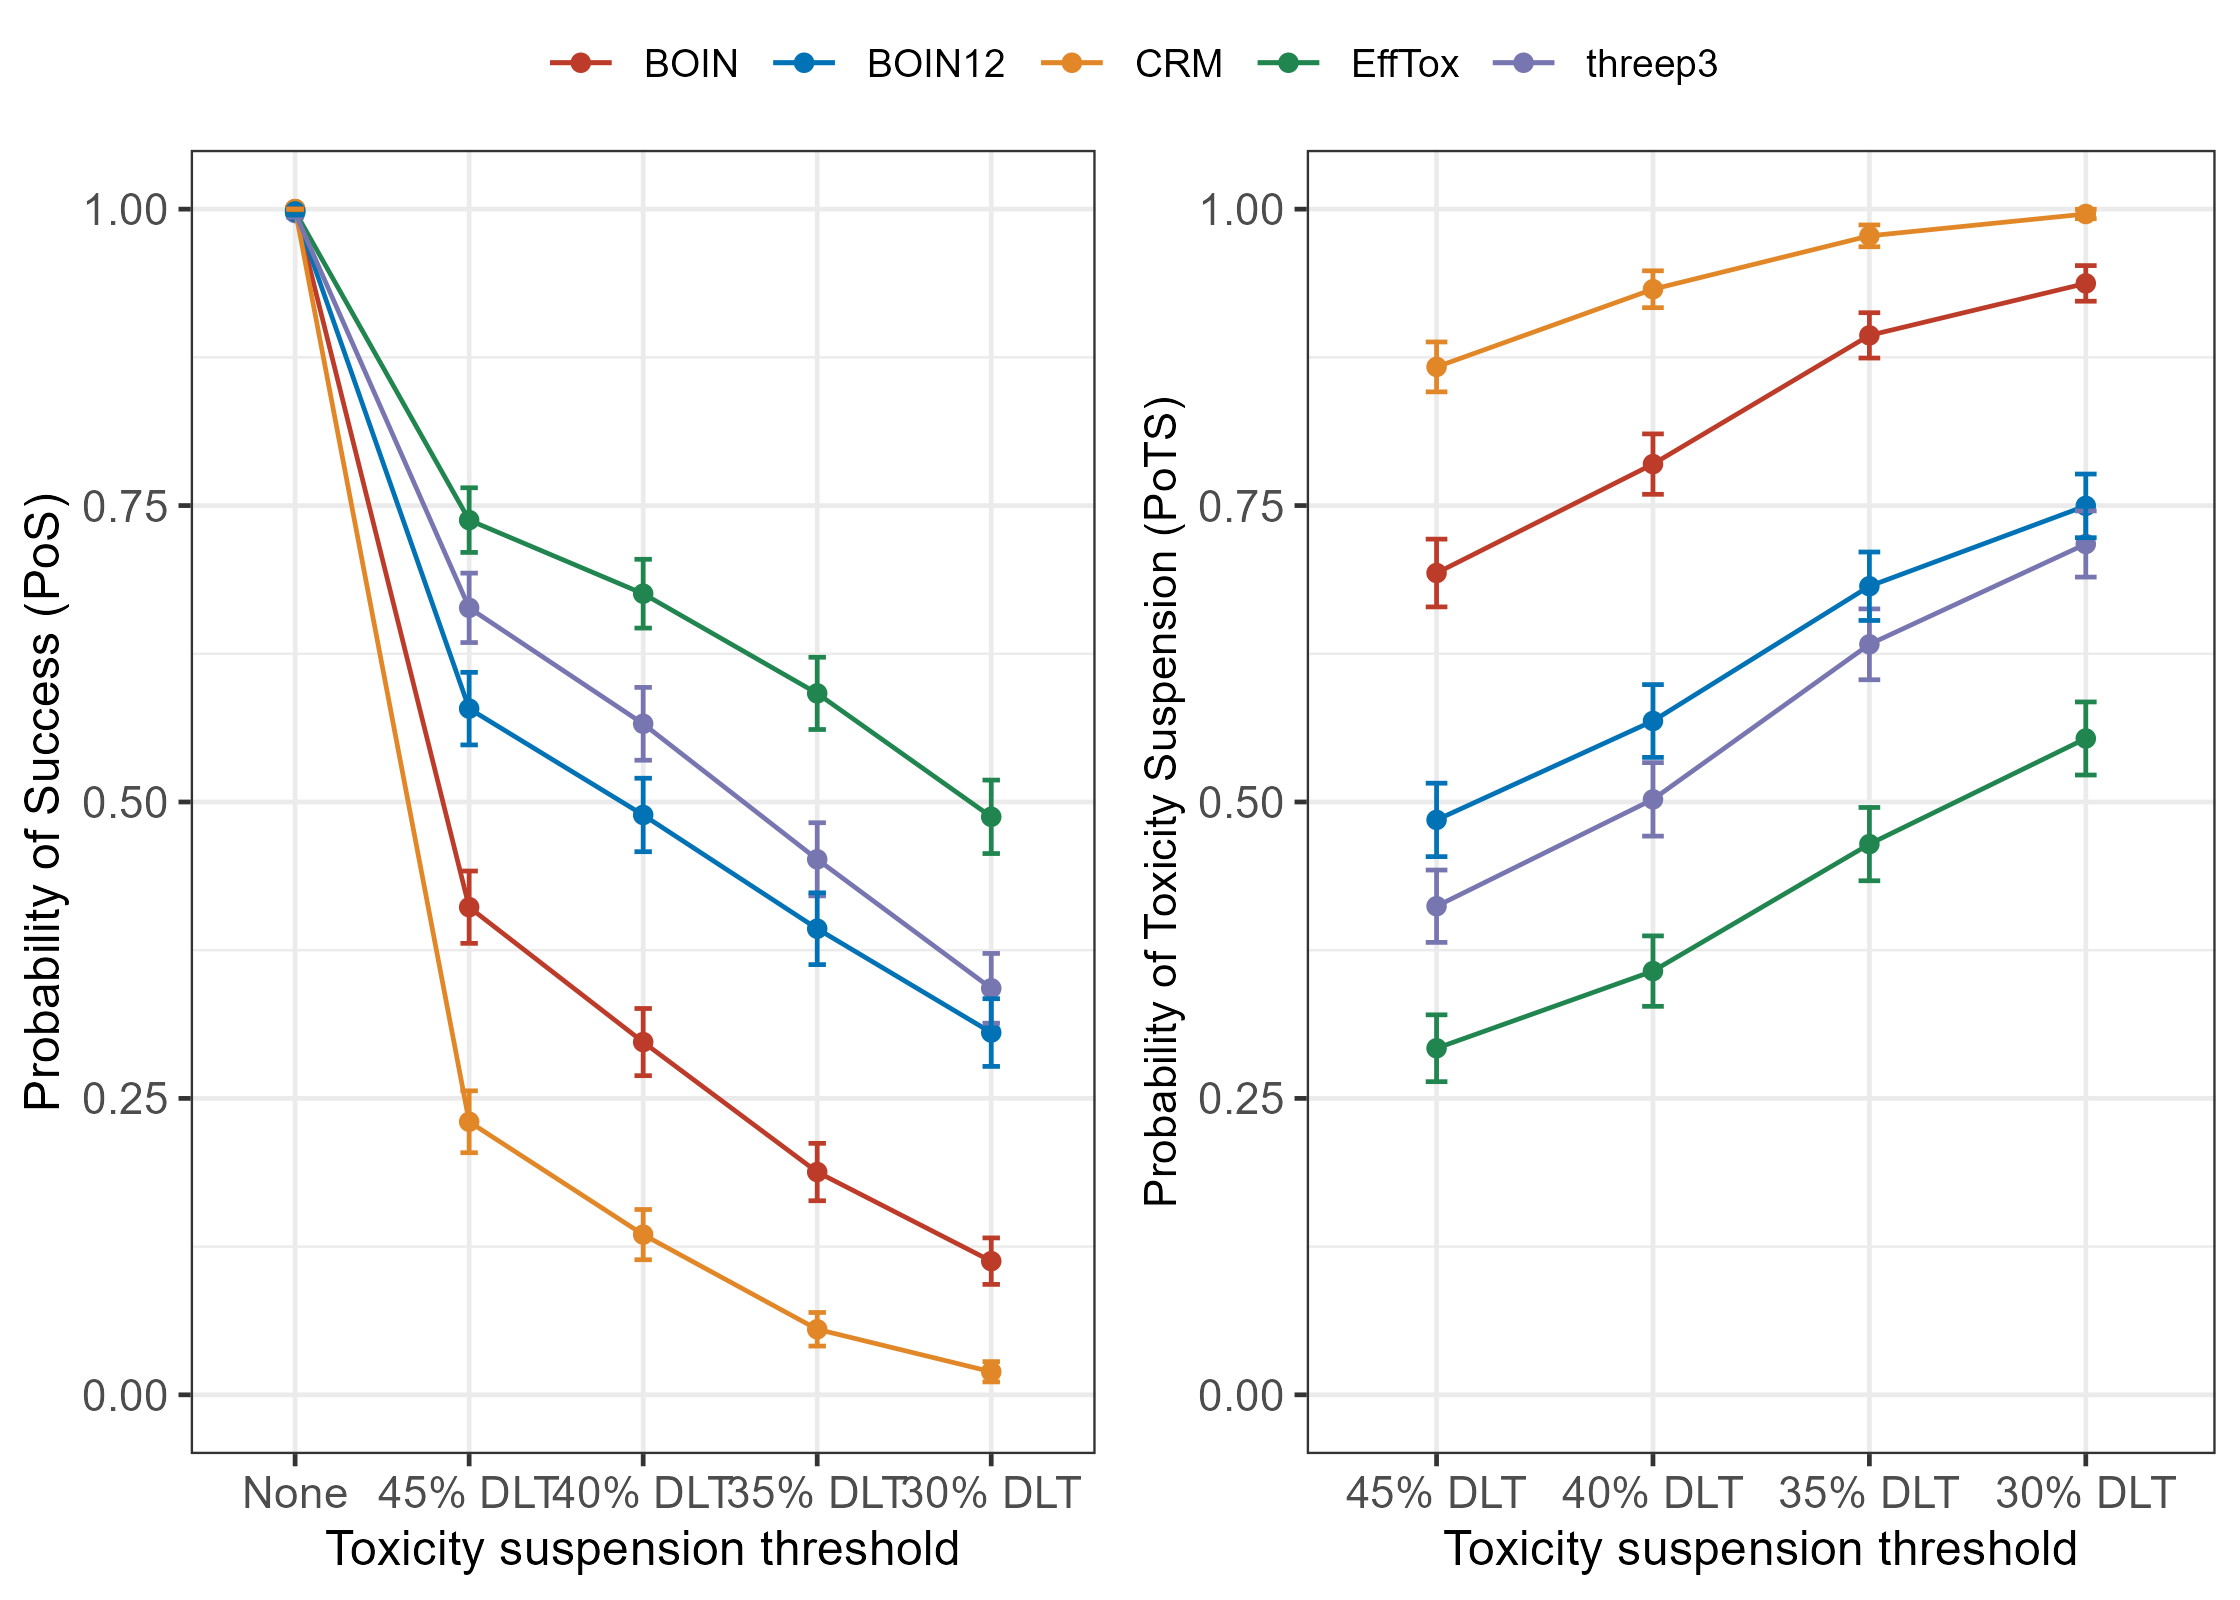
\includegraphics[width=0.8\textwidth]{plots/plot_Imatinib.png}
    \caption{Probability of overall success (PoS) (left) and probability of toxicity suspension (PoTS) (right) across different Phase I dose-finding designs and late-phase toxicity control settings for Imatinib. The error bars represent 95\% Monte Carlo confidence intervals.}
    \label{plot-Imatinib}
\end{figure}

\section{Discussion}
This simulation study examined how Phase I dose-finding methods influence the probability of overall drug development success across a range of drug profiles and late-phase toxicity control rules. For chemotherapy-like profiles where the MTD is a proper dosing target, BOIN and CRM consistently outperformed 3+3, which agrees with previous studies \parencite{conaway2019impact,ruppert2018overall}. Bivariate designs added limited benefit despite incorporating early efficacy data. This is expected because efficacy increases monotonically with dose for cytotoxic agents, making toxicity-driven dose escalation sufficient for identifying clinically effective doses. Moreover, the additional model complexity introduced by modeling both efficacy and toxicity may reduce efficiency in small-sample Phase I settings. 

In contrast, for immunotherapy-like profiles, the advantages of more efficient univariate methods over 3+3 were compromised, especially under stricter toxicity control. In these scenarios, targeting the MTD rather than the OBD resulted in unnecessary toxicity that was increasingly penalized in later phases. Bivariate designs therefore achieved more robust overall success rates by better balancing efficacy and toxicity during dose selection. However, bivariate designs require additional specifiction of utility parameters compared to univariate designs, which can add extra implementation complexity. In align with previous findings \parencite{BOIN12}, our sensitivity analyses indicated that the performance of EffTox was more sensitive utility specfication compared to BOIN12. The robustness of BOIN12 to utility specification may facilitate real-world implementation compared to EffTox. Notably, although 3+3 occasionally achieved comparable or even superior downstream performance in certain scenarios, these results appeared largely driven by its inherently conservative escalation behavior rather than by appropriate targeting of the underlying dose profile. Such favorable performance is therefore unlikely to generalize reliably across settings. Consequently, we would still recommend the use of more statistically efficient designs, together with thorough consideration of the anticipated drug profile, rather than relying on the 3+3 design.

The steeper decline in PoS with stricter toxicity suspension thresholds for chemotherapy-like profiles reflects their monotonic dose-efficacy relationships: doses near the MTD are often either subtherapeutic or excessively toxic, so dose mis-selection carries a large penalty and leaves less room for downstream success. In contrast, immunotherapy-like profiles typically plateau around the OBD, meaning adjacent doses retain comparable efficacy and differ mainly by unnecessary toxicity. Consequently, modest dose mis-selection does not severely compromise efficacy, leading to greater downstream robustness. Therefore, downstream simulation is particularly valuable when prior knowledge on the underlying drug profile is limited or when stringent toxicity monitoring is anticipated in later trial phases, as under these conditions accurate MTD identification may not directly translate into higher PoS. 

This study has several limitations. First, we considered only a limited set of drug profiles and representative Phase I designs. We also investigated a single, typical sample size in Phase I. In addition, toxicity assessment in the main simulations was primarily based on short-term DLT outcomes, which may not fully capture the long-term safety profile of a treatment. The Imatinib example highlights this limitation: an RP2D selected using early DLT data alone may exceed the true OBD because later cumulative or delayed toxicities are not yet observable during the Phase I evaluation window. As a result, doses that initially appear tolerable may subsequently lead to substantial toxicity burden and increased trial suspension rate in later phases. For agents with delayed or cumulative toxicities, methods that incorporate long-term toxicity and efficacy information, such as TITE-BOIN12, may be preferable \parencite{TITE-BOIN12}. Second, our late-phase trial models are simplified and do not capture the full complexity of real-world development. For example, we did not model dose modifications, treatment discontinuation, or more sophisticated safety monitoring in Phase II and III, all of which could mitigate the downstream impact of aggressive Phase I dose selection. We also made quite a strong assumption that the underlying survival distribution is exponential such that we could generate survival data based on reported median survival times.

In summary, downstream success depends strongly on the shape of the underlying drug profile. These findings underline the importance of understanding the potential shape of the candidate drug profile from pre-clinical studies when designing early-phase trials. We propose a flexible simulation pipeline for methodological comparison. Future work could utilize this fraevaluate the impact of carrying multiple doses into Phase II and other novel adaptive early-phase designs, such as seamless Phase I/II trials and platform trials.


\newpage
\addcontentsline{toc}{section}{Reference}
\section*{Reference}
\printbibliography [heading=none]

\appendix
\renewcommand{\thefigure}{S\arabic{figure}}
\setcounter{figure}{0}
\renewcommand{\thetable}{S\arabic{table}}
\setcounter{table}{0}
\newpage
\section*{Appendix}
\subsection*{Imatinib example data generation}
The data generation is divided into two steps. 

In step 1, we generate the exposure data for the patient cohort based on their relevant pharmacological characteristics: the white blood cell count (WBC) and albumin level (ALB) that affects drug absorption and clearance. WBC and ALB are generated from a bivariate normal distribution with mean of 5.59 $(10^9/L)$ and 35.5 $(g/L)$, standard deviation of 1.86 and 5.0, and correlation of -0.5, based on the observed distribution in the clinical trial data. The exposure outcome is $C_{min}$, defined as the trough concentration of drug in the plasma during a repeated dosing regimen, i.e. the drug concentration immediately prior to the administration of a subsequent dose. We use $C_{min}$ at steady state (240 hours from first dosing). The one-compartment PK model from \textcite{demetri2009imatinib} is adopted to relate the simulated WBC and ALB to $C_{min}$ under different doses of Imatinib. The distribution of simulated $C_{min}$ values for each dose is shown in Figure \ref{Dist-Imatinib-Cmin}.

In step 2,  we map the simulated exposure to clinical outcomes via the constructed exposure-toxicity, exposure-response, exposure-PFS (progression-free survival) curves. There is little information on the exposure-toxicity relationship of Imatinib in the literature, besides that a $C_{min}$ of 3180 $ug/L$ is usually considered as the threshold for toxicity. We therefore assume a logistic-type relationship between $C_{min}$ and the probability of DLT $p_{DLT}$

$$p_{DLT}(C_{min}) = \frac{L}{(1+e^{-Z_1})+(1-e^{-Z_2})}, Z_1 = a+k\cdot \frac{C_{min}}{1000}, Z_2 = a+k\cdot \frac{C_{max}}{1000},$$

with $L=0.5, a=-5.5, k=2, C_{max}=4200$ for short-term DLT in Phase I and $L=0.95, a=-4.5, k=1.86, C_{max}=4200$ for long-term DLT in Phase II and III. These parameters are tuned such that the probability of DLT at $C_{min}=3180$ is around 37\% for Phase I and 79\% for Phase II and III.

The exposure-response relationship is constructed based on the observed tumor response rates (TRR) at three quantiles of $C_{min}$ reported in the literature \parencite{demetri2009imatinib}. We assume the following functional form to allow the TRR to increase with drug exposure in a monotonic, saturating manner

$$TRR(C_{min}) = TRR_{max} \cdot \frac{1-\exp (-kC_{min})}{1-\exp (-kC_{max})},$$

with $TRR_{max}=0.7, k=1.05, C_{max}=4200$.

The exposure-PFS relationship is constructed based on the observed median PFS at the same three quantiles of $C_{min}$ \parencite{demetri2009imatinib}. We assume an expenential decrease in the hazard of progression with increasing drug exposure, with the following functional form

$$h(C_{min}) = a \cdot \exp (bC_{min})+h_{min},$$

with $a=0.15, b=-0.004, h_{min}=0.03$. Then the PFS is modeled by an exponential distribution with the corresponding hazard. The reason for including a non-zero $h_{min}$ is to prevent unrealistic large PFS values. 

We compare the simulated outcome summaries with the outcome summaries reported from different trials. We have very limited data from the Phase I as it evaluated only 40 patients. One key difference between the DLT rate observed in Phase I trial and that observed in Phase II/III trials is the time window. Phase I assessed short-term DLT that occurred during the first 8 weeks after randomization while later phases recorded DLT/dose reduction during the whole follow-up. From Table \ref{Imatinib_ST_DLT_comparison} we can conclude the simulated short-term DLT is not very extreme for all dose levels. The simulated long-term DLT rate for dose 400 mg align reasonably with both Phase II and Phase III statistics. The simulated long-termDLT rate for 600 mg is a bit above the 95\% confidence interval for the DLT rate reported in Phase II trial. The simulated long-term DLT rate is a bit low for dose 800 mg (Table \ref{Imatinib_LT_DLT_comparison}). It is a bit difficult to say whether the simulated response rates align with the reported response rate, because the reported response rates from Phase II and III differ a lot (Table \ref{Imatinib_TRR_comparison}). In trial reports, the PFS did not differ significantly whether comparing 400 mg vs. 600 mg or 400 mg vs. 800 mg, indicating that the survival might be quite similar across the four doses, which is reflected in the simulated data (Table \ref{Imatinib_PFS_comparison}).

\begin{table}[htbp]
\centering
\caption{Comparison of simulated short-term DLT rates with reported short-term DLT rates from Phase I trial under doses 400, 600, 800, and 1000 mg.}
\label{Imatinib_ST_DLT_comparison}
\begin{tabular}{lll}
\toprule
\textbf{Dose (mg)} & \textbf{Simulated} & \textbf{Phase 1, Oosterom et al.} \\
\midrule
400  & 0.099 & 0 (0--0.37) \\
600  & 0.203 & 0.25 (0.03--0.65) \\
800  & 0.294 & 0.06 (0--0.30) \\
1000 & 0.364 & 0.75 (0.35--0.97) \\
\bottomrule
\end{tabular}
\end{table}

\begin{table}[htbp]
\centering
\caption{Comparison of simulated long-term DLT rates with reported long-term DLT rates from Phase II \& III trials under doses 400, 600, 800, and 1000 mg. NA indicates the dose was not investigated.}
\label{Imatinib_LT_DLT_comparison}
\begin{tabular}{llll}
\toprule
\textbf{Dose (mg)} & \textbf{Simulated} & \textbf{Phase II, Blanke et al.} & \textbf{Phase III, Blanke et al.} \\
\midrule
400  & 0.185 & 0.21 (0.12--0.32) & 0.16 (0.12--0.20) \\
600  & 0.344 & 0.22 (0.13--0.33) & NA \\
800  & 0.482 & NA & 0.58 (0.52--0.63) \\
1000 & 0.59  & NA & NA \\
\bottomrule
\end{tabular}
\end{table}

\begin{table}[htbp]
\centering
\caption{Comparison of simulated response rates with reported response rates from different sources under doses 400, 600, 800, and 1000 mg. NA indicates the dose was not investigated in the trial.}
\label{Imatinib_TRR_comparison}
\begin{tabular}{llll}
\toprule
\textbf{Dose (mg)} & \textbf{Simulated} & \textbf{Phase II, Blanke et al.} & \textbf{Phase III, Blanke et al.} \\
\midrule
400  & 0.472 & 0.69 (0.57--0.79) & 0.45 (0.39--0.50) \\
600  & 0.549 & 0.65 (0.56--0.78) & NA \\
800  & 0.595 & NA & 0.46 (0.41--0.51) \\
1000 & 0.624 & NA & NA \\
\bottomrule
\end{tabular}
\end{table}

\begin{table}[htbp]
\centering
\caption{Comparison of simulated median PFS with reported median PFS from different sources under doses 400, 600, 800, and 1000 mg. NA indicates the dose was not investigated in the trial.}
\label{Imatinib_PFS_comparison}
\begin{tabular}{llll}
\toprule
\textbf{Dose (mg)} & \textbf{Simulated} & \textbf{Phase II, Blanke et al.} & \textbf{Phase III, Blanke et al.} \\
\midrule
400  & 18.7 & 20 (16--29) & 18 (16--21) \\
600  & 20.9 & 26 (16--41) & NA \\
800  & 21.6 & NA & 20 (17--25) \\
1000 & 22.2 & NA & NA \\
\bottomrule
\end{tabular}
\end{table}

\newpage
\subsection*{Supplementary figures}
\begin{figure}[htbp]
    \centering
    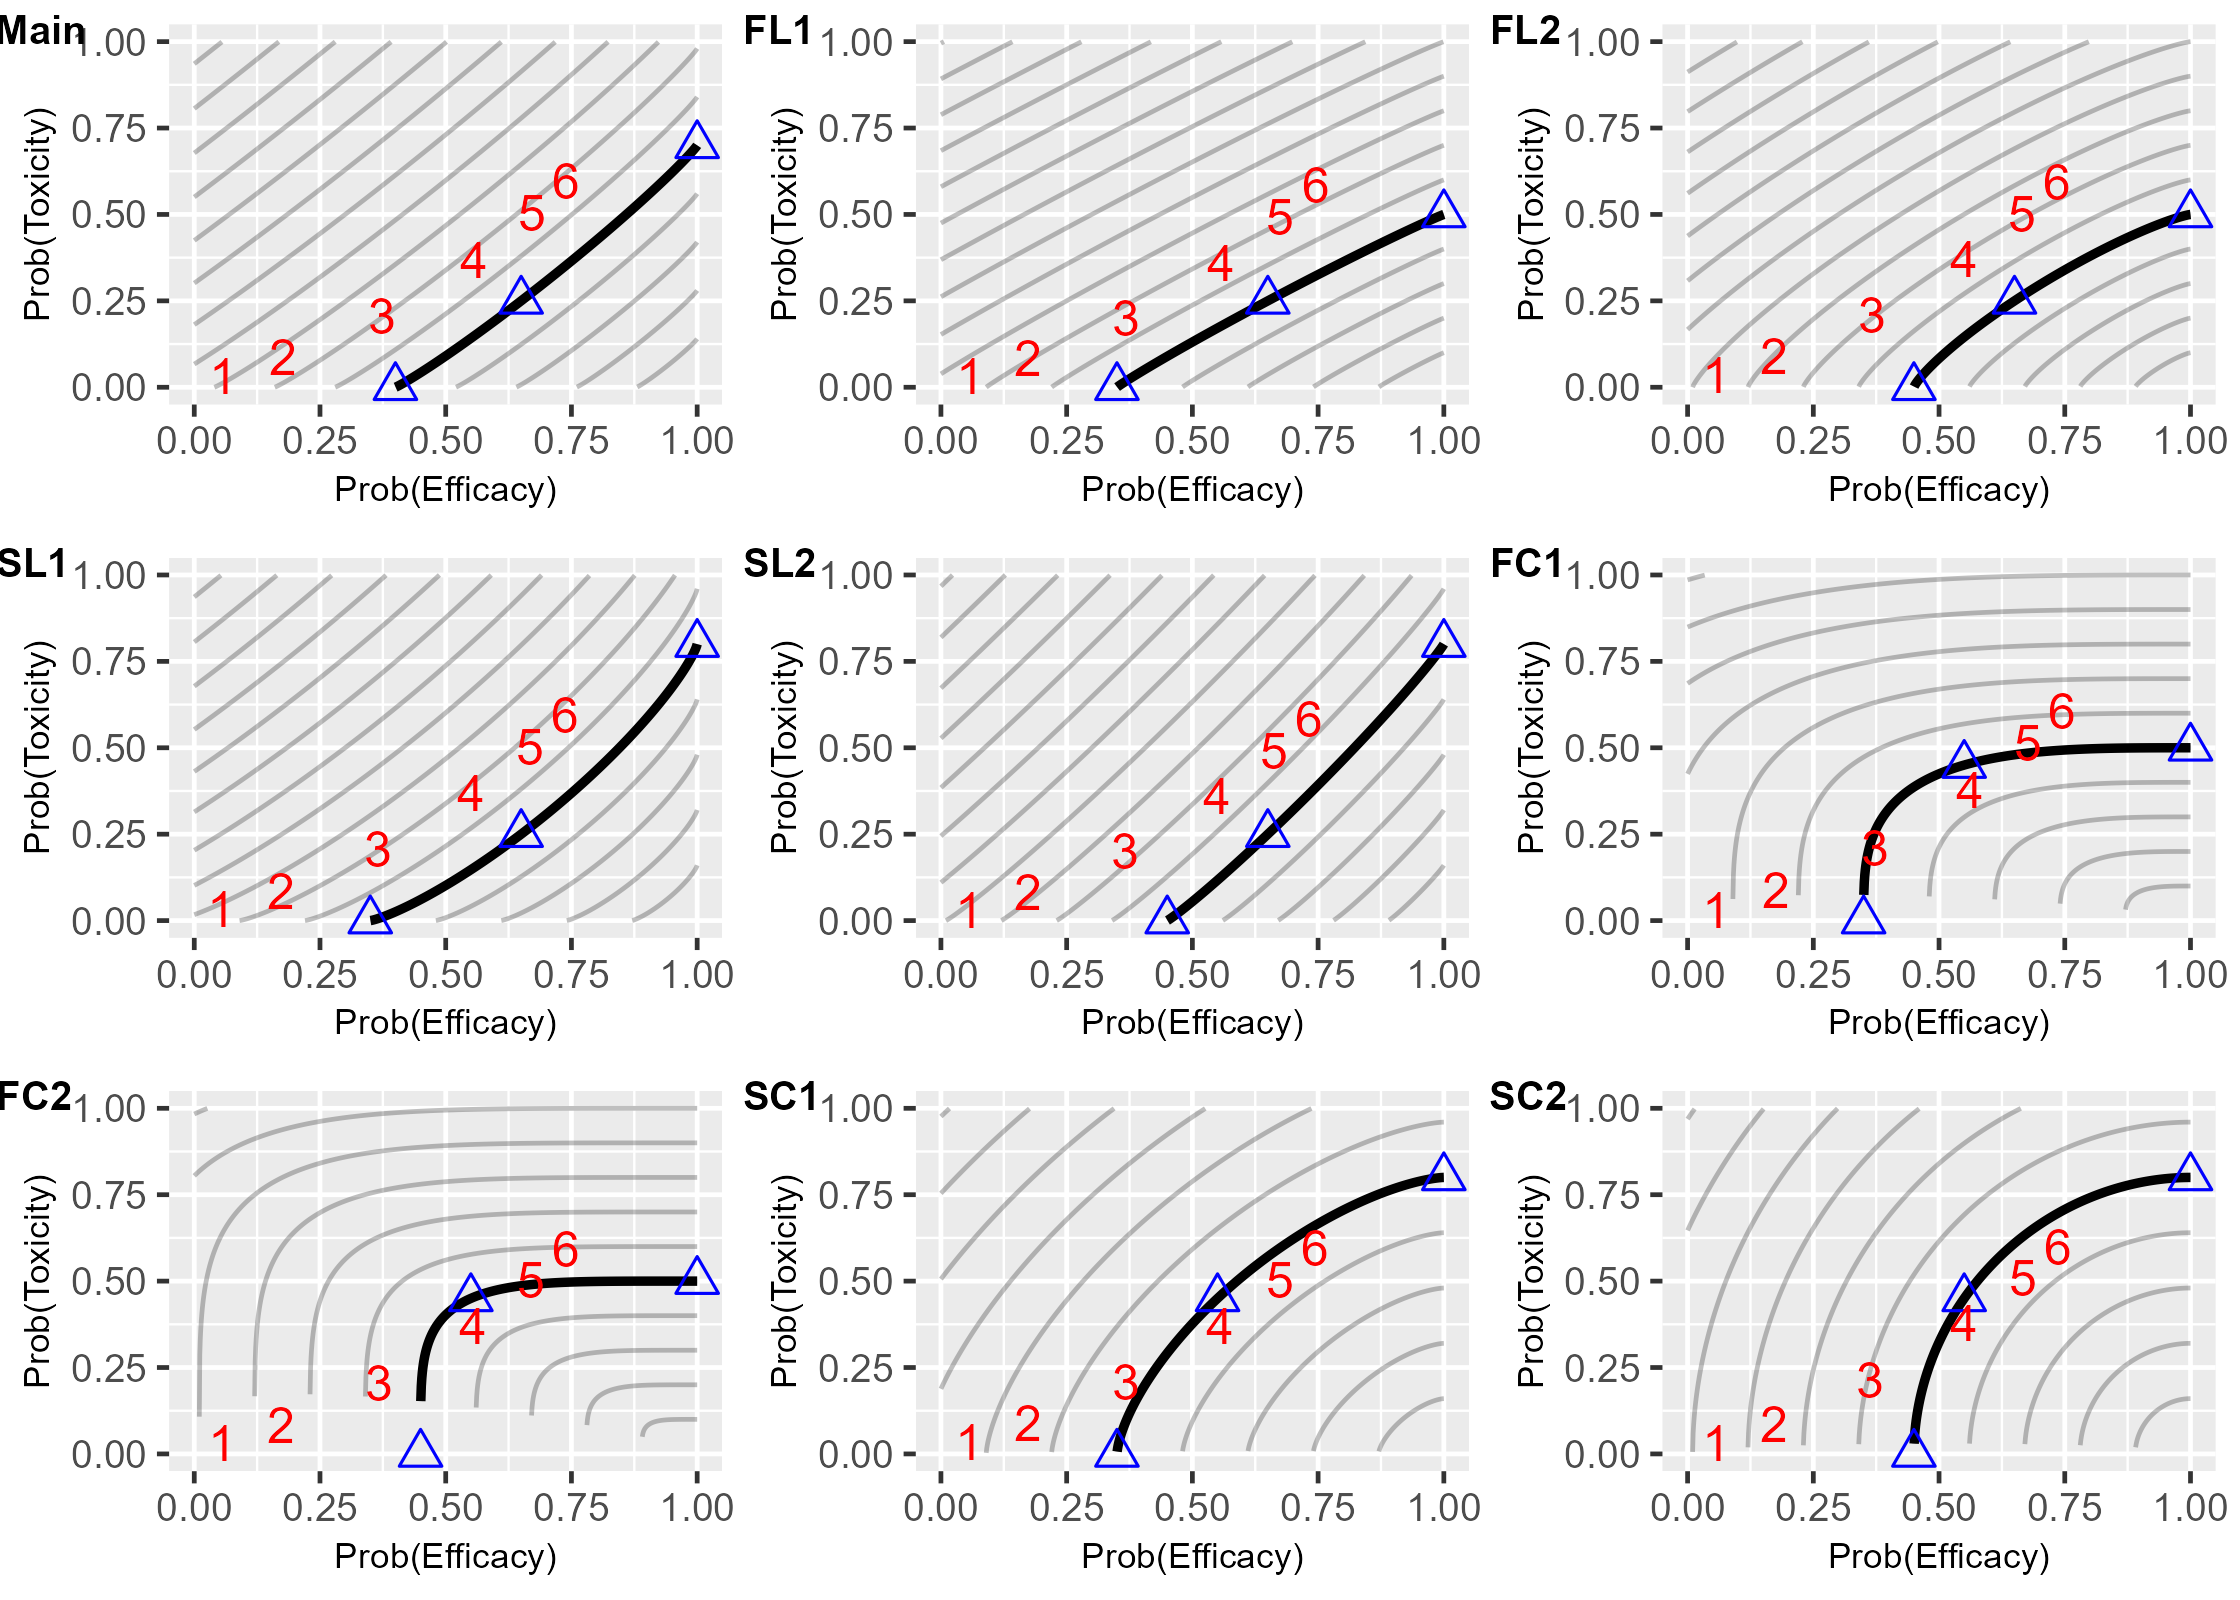
\includegraphics[width=0.9\textwidth]{plots/supplement/EffTox_contour.png}
    \caption{Contour plots used in the sensitivity analysis of EffTox. Main: used in the main simulation.}
    \label{plot-EffTox-Contour}
\end{figure}

\begin{figure}[htbp]
    \centering
    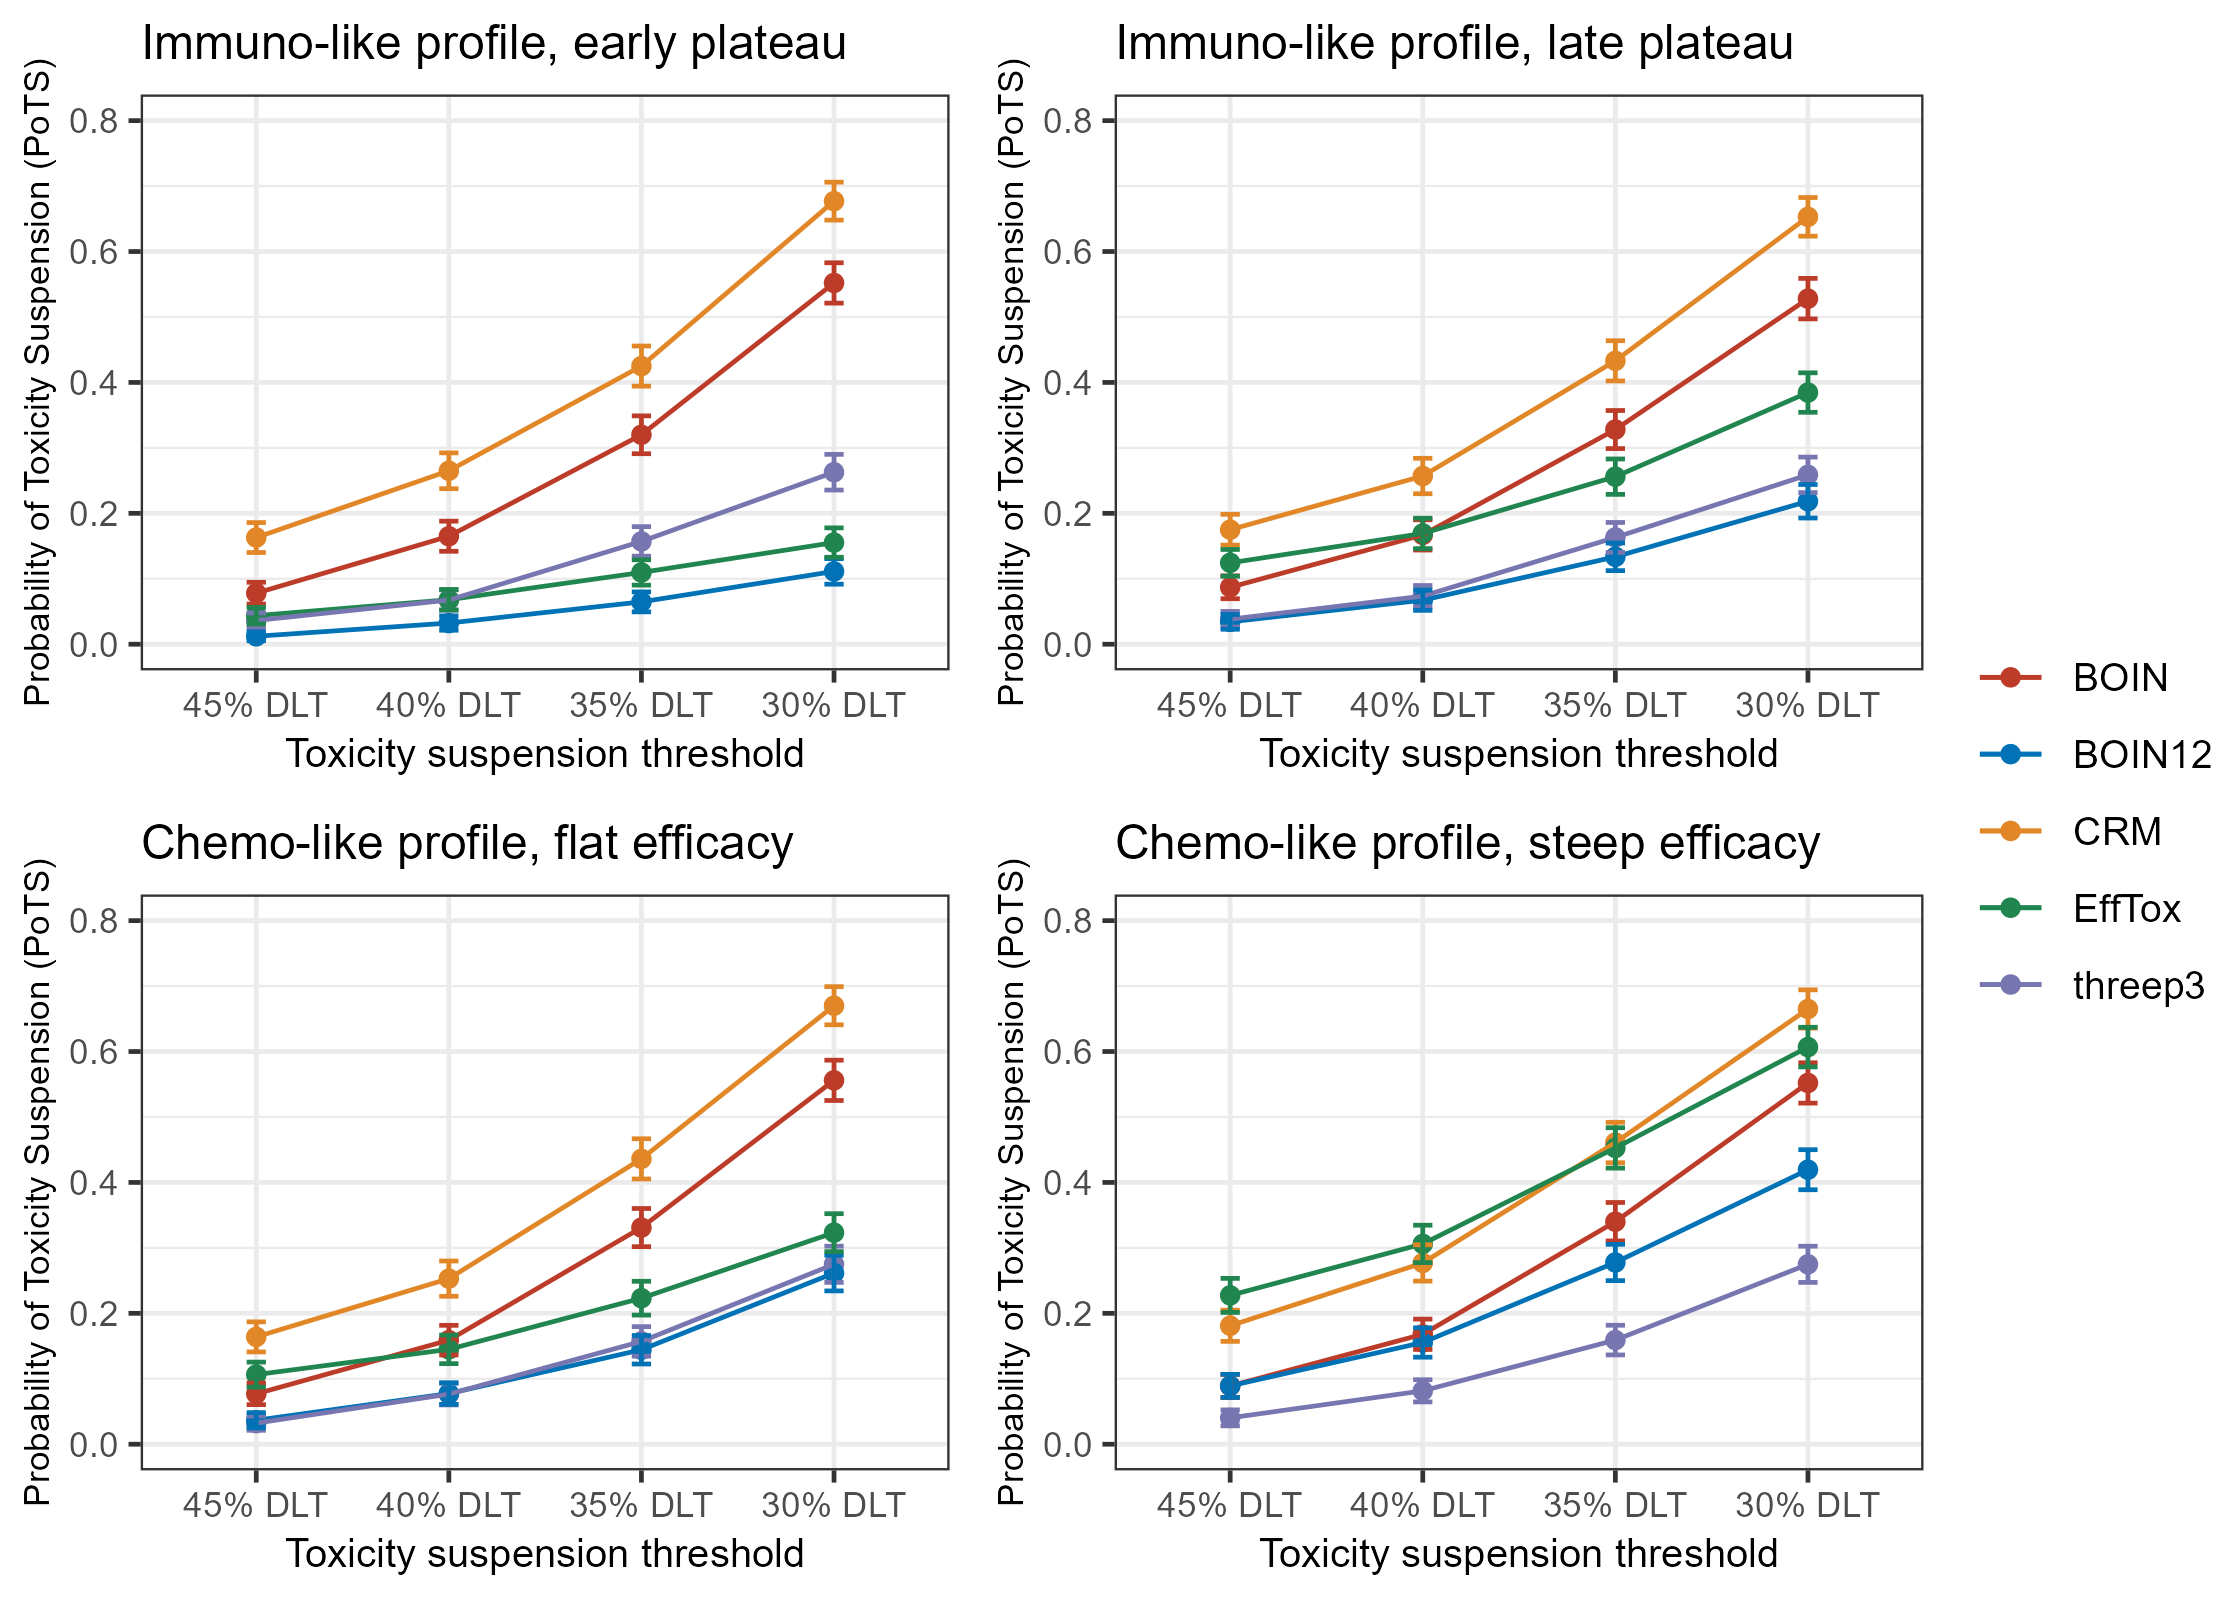
\includegraphics[width=0.9\textwidth]{plots/supplement/plot_PoTS.png}
    \caption{Probability of Toxicity Suspension (PoTS) across different Phase I dose-finding methods and late-phase toxicity control settings for chemotherapy-like and immunotherapy-like drug profiles. The error bars represent 95\% Monte Carlo confidence intervals.}
    \label{plot-PoTS}
\end{figure}

\begin{figure}[htbp]
    \centering
    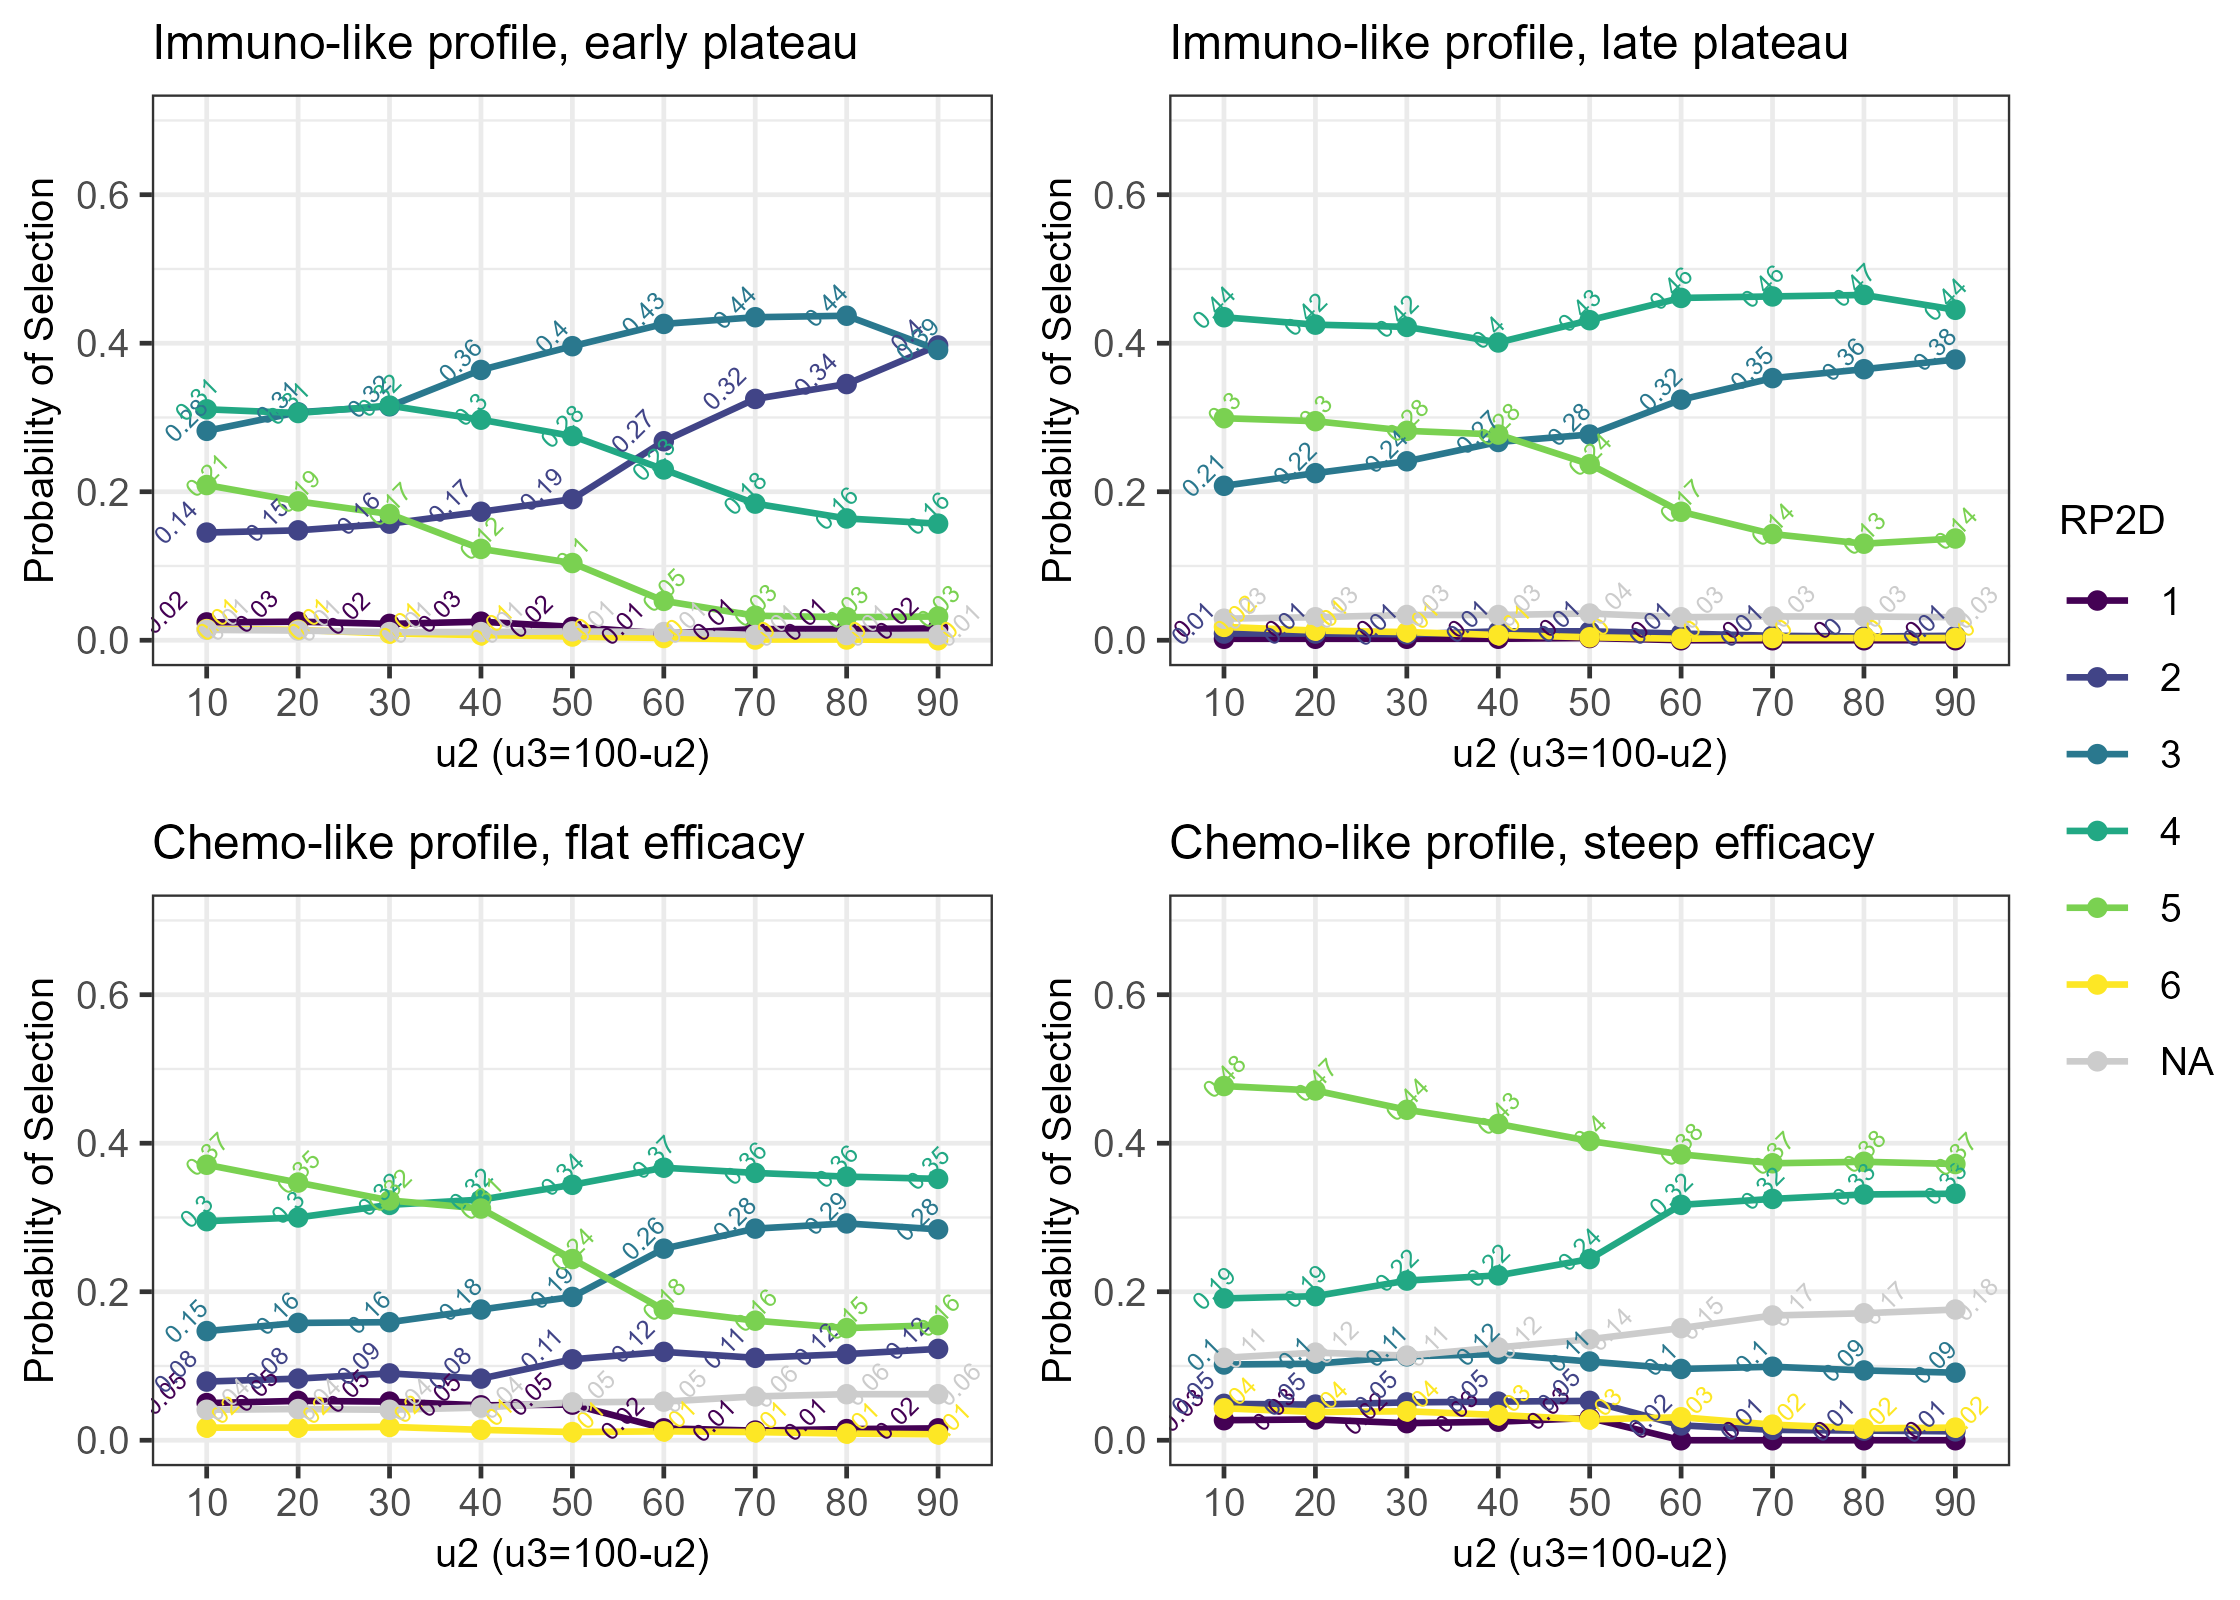
\includegraphics[width=0.9\textwidth]{plots/supplement/sens_BOIN12_RP2D.png}
    \caption{Probability of selecting each dose as the RP2D across 1000 simulated Phase I trials for BOIN12 with varying values of $u_2$}
    \label{plot-sens-BOIN12-RP2D}
\end{figure}

\begin{figure}
    \centering
    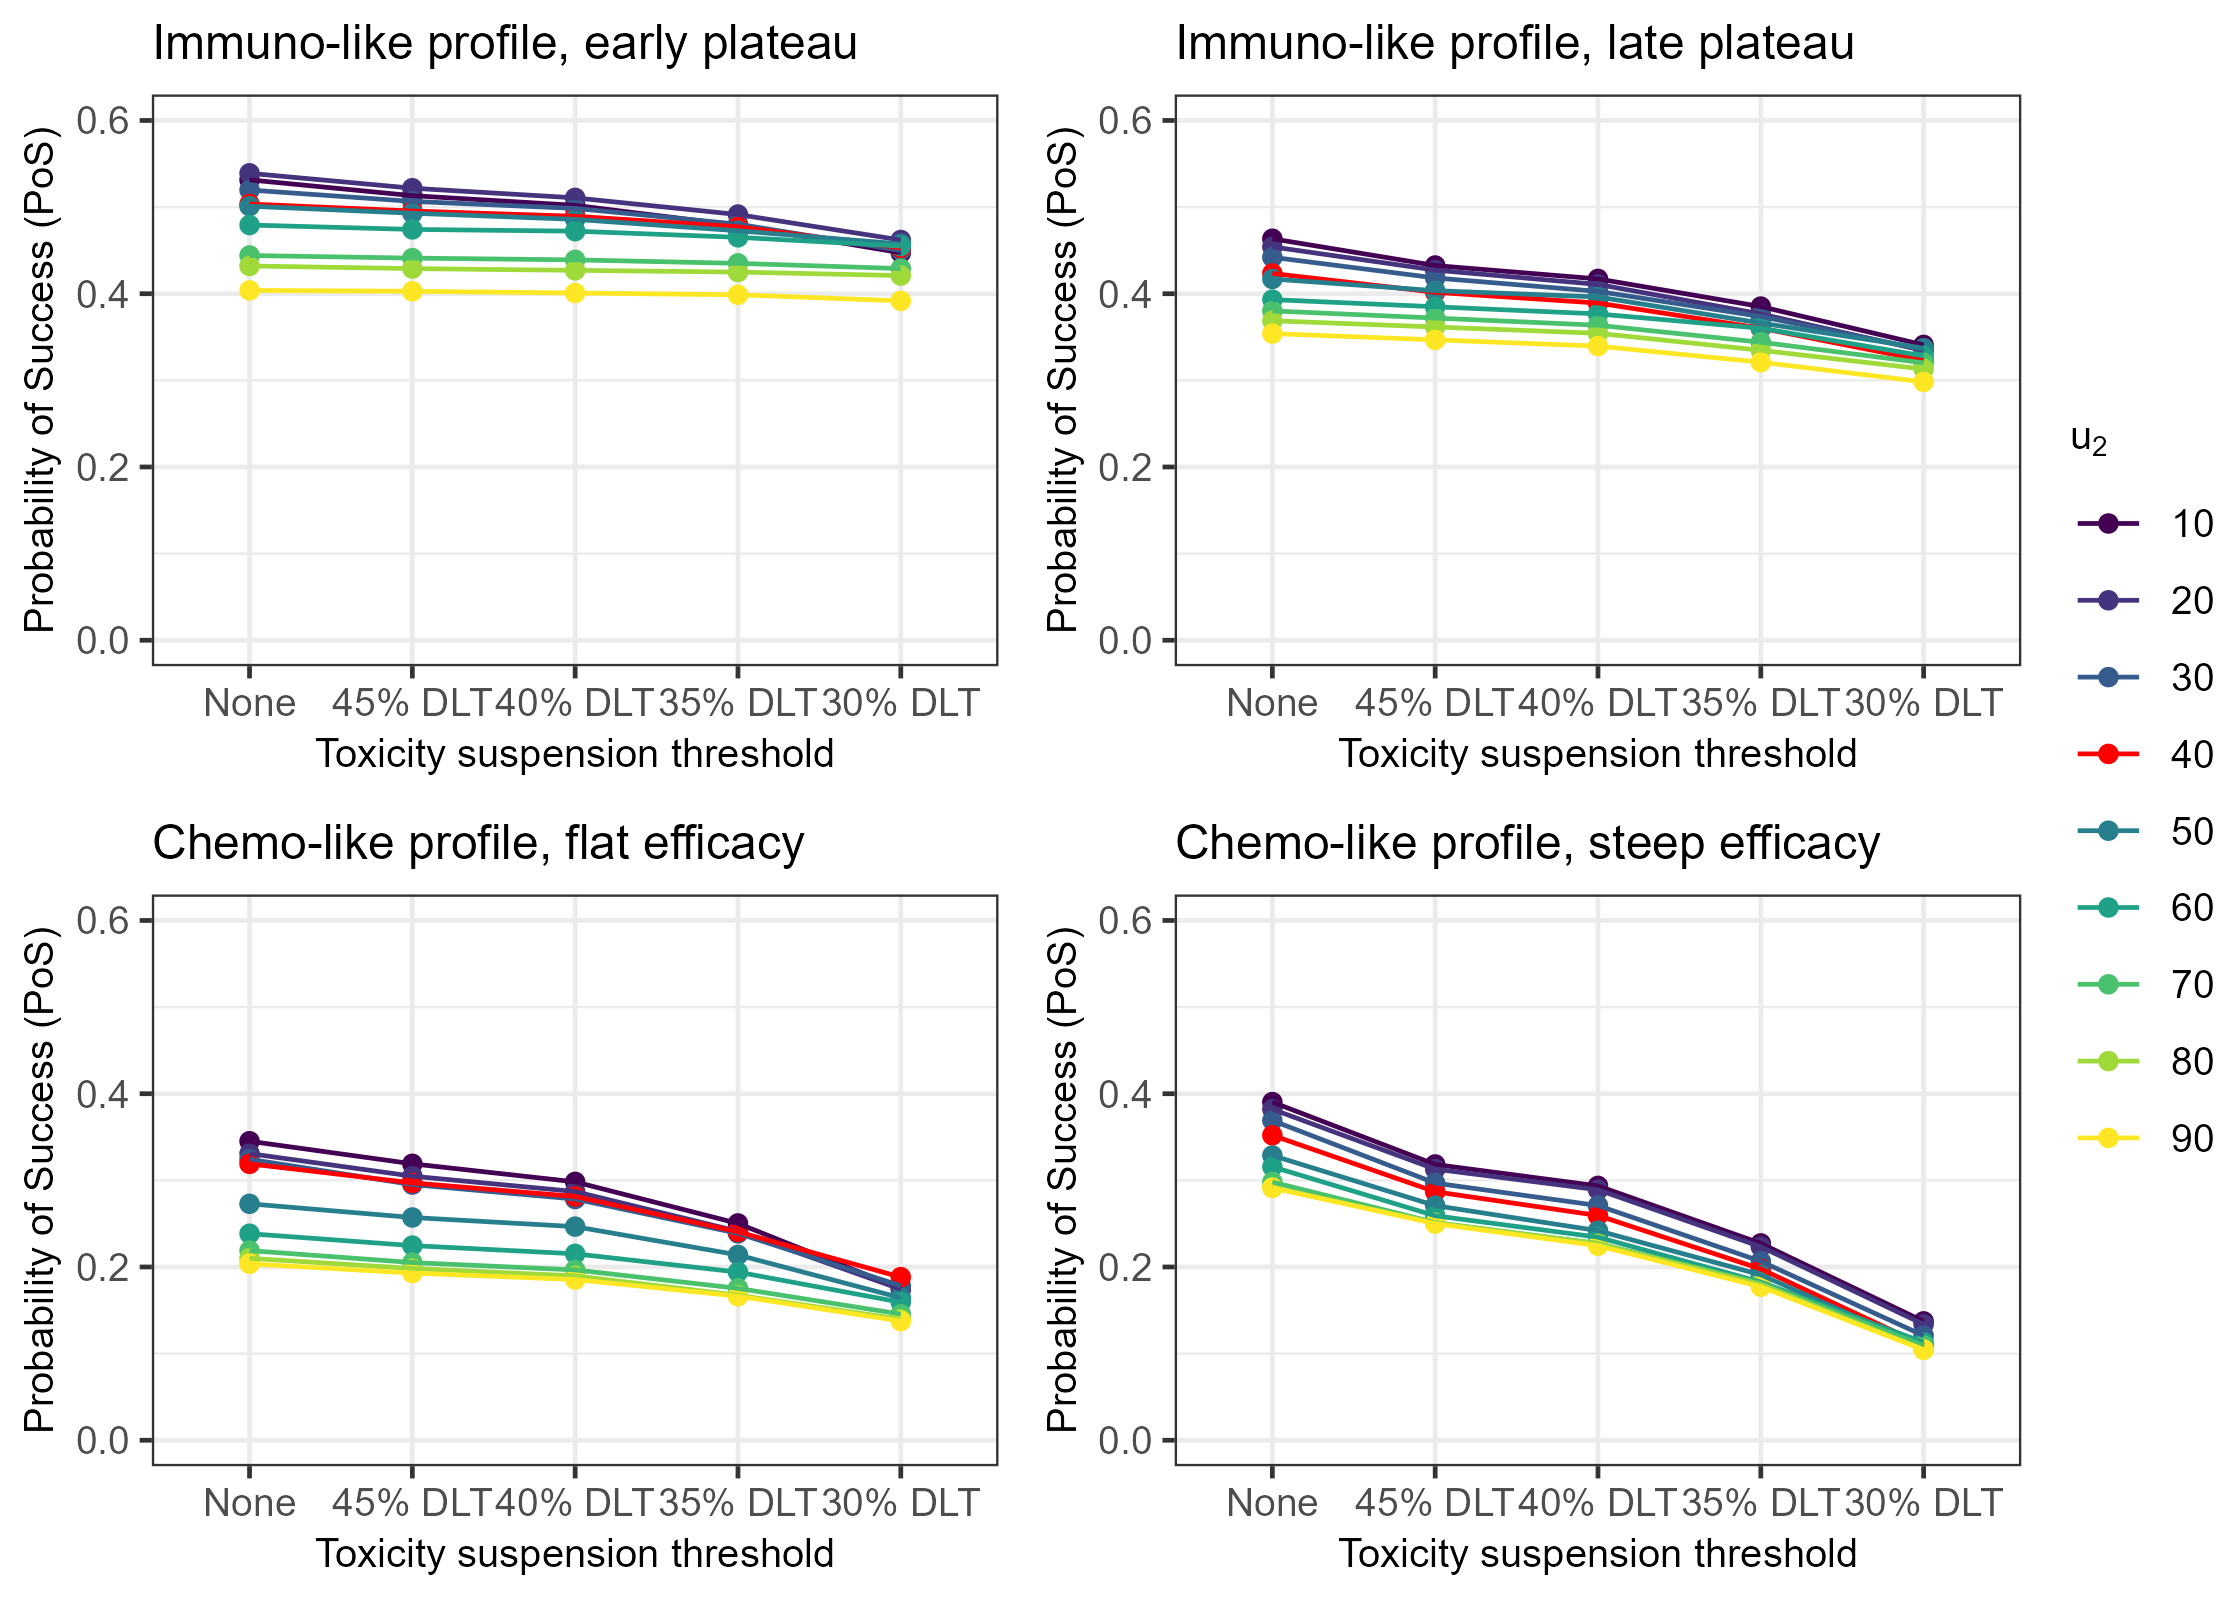
\includegraphics[width=0.9\textwidth]{plots/supplement/sens_BOIN12_PoS.png}
    \caption{Probability of overall success (PoS) of BOIN12 across different values of $u_2$ for chemotherapy-like and immunotherapy-like drug profiles. The red line represents the result from the main simulation.}
    \label{plot-sens-BOIN12-PoS}
\end{figure}

\begin{figure}[htbp]
    \centering
    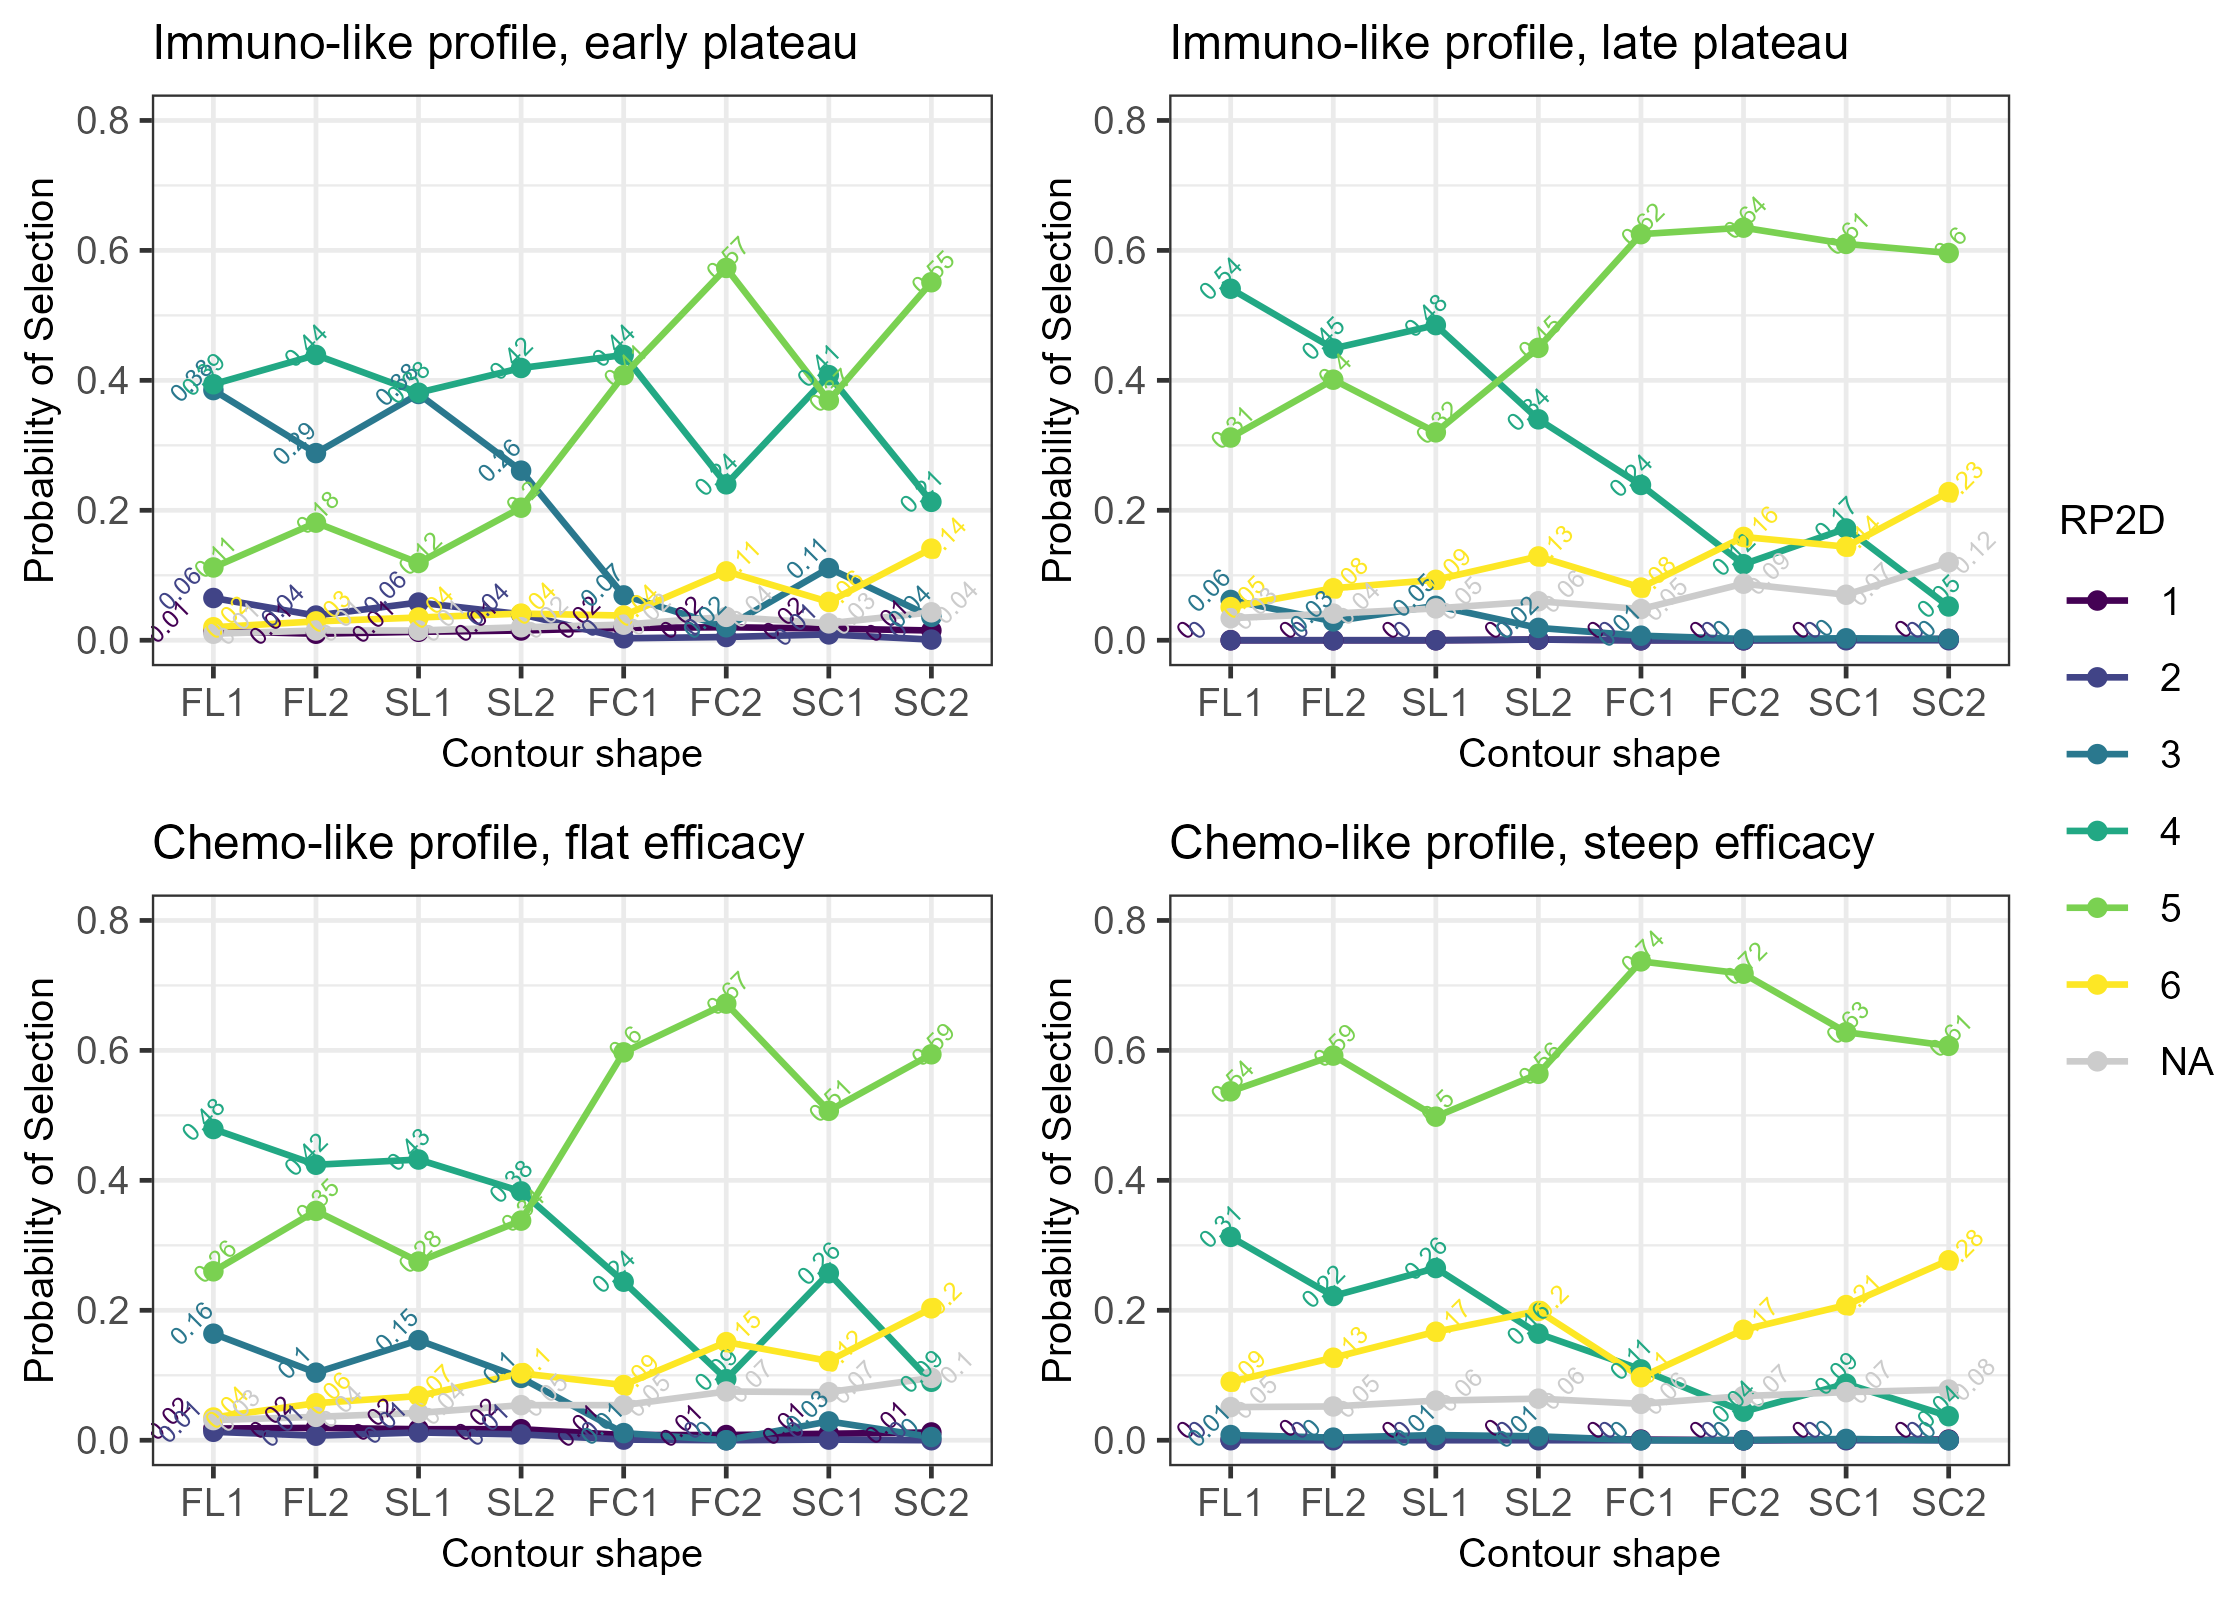
\includegraphics[width=0.9\textwidth]{plots/supplement/sens_EffTox_RP2D.png}
    \caption{Probability of selecting each dose as the RP2D across 1000 simulated Phase I trials for EffTox with different contour specifications.}
    \label{plot-sens-EffTox-RP2D}
\end{figure}

\begin{figure}
    \centering
    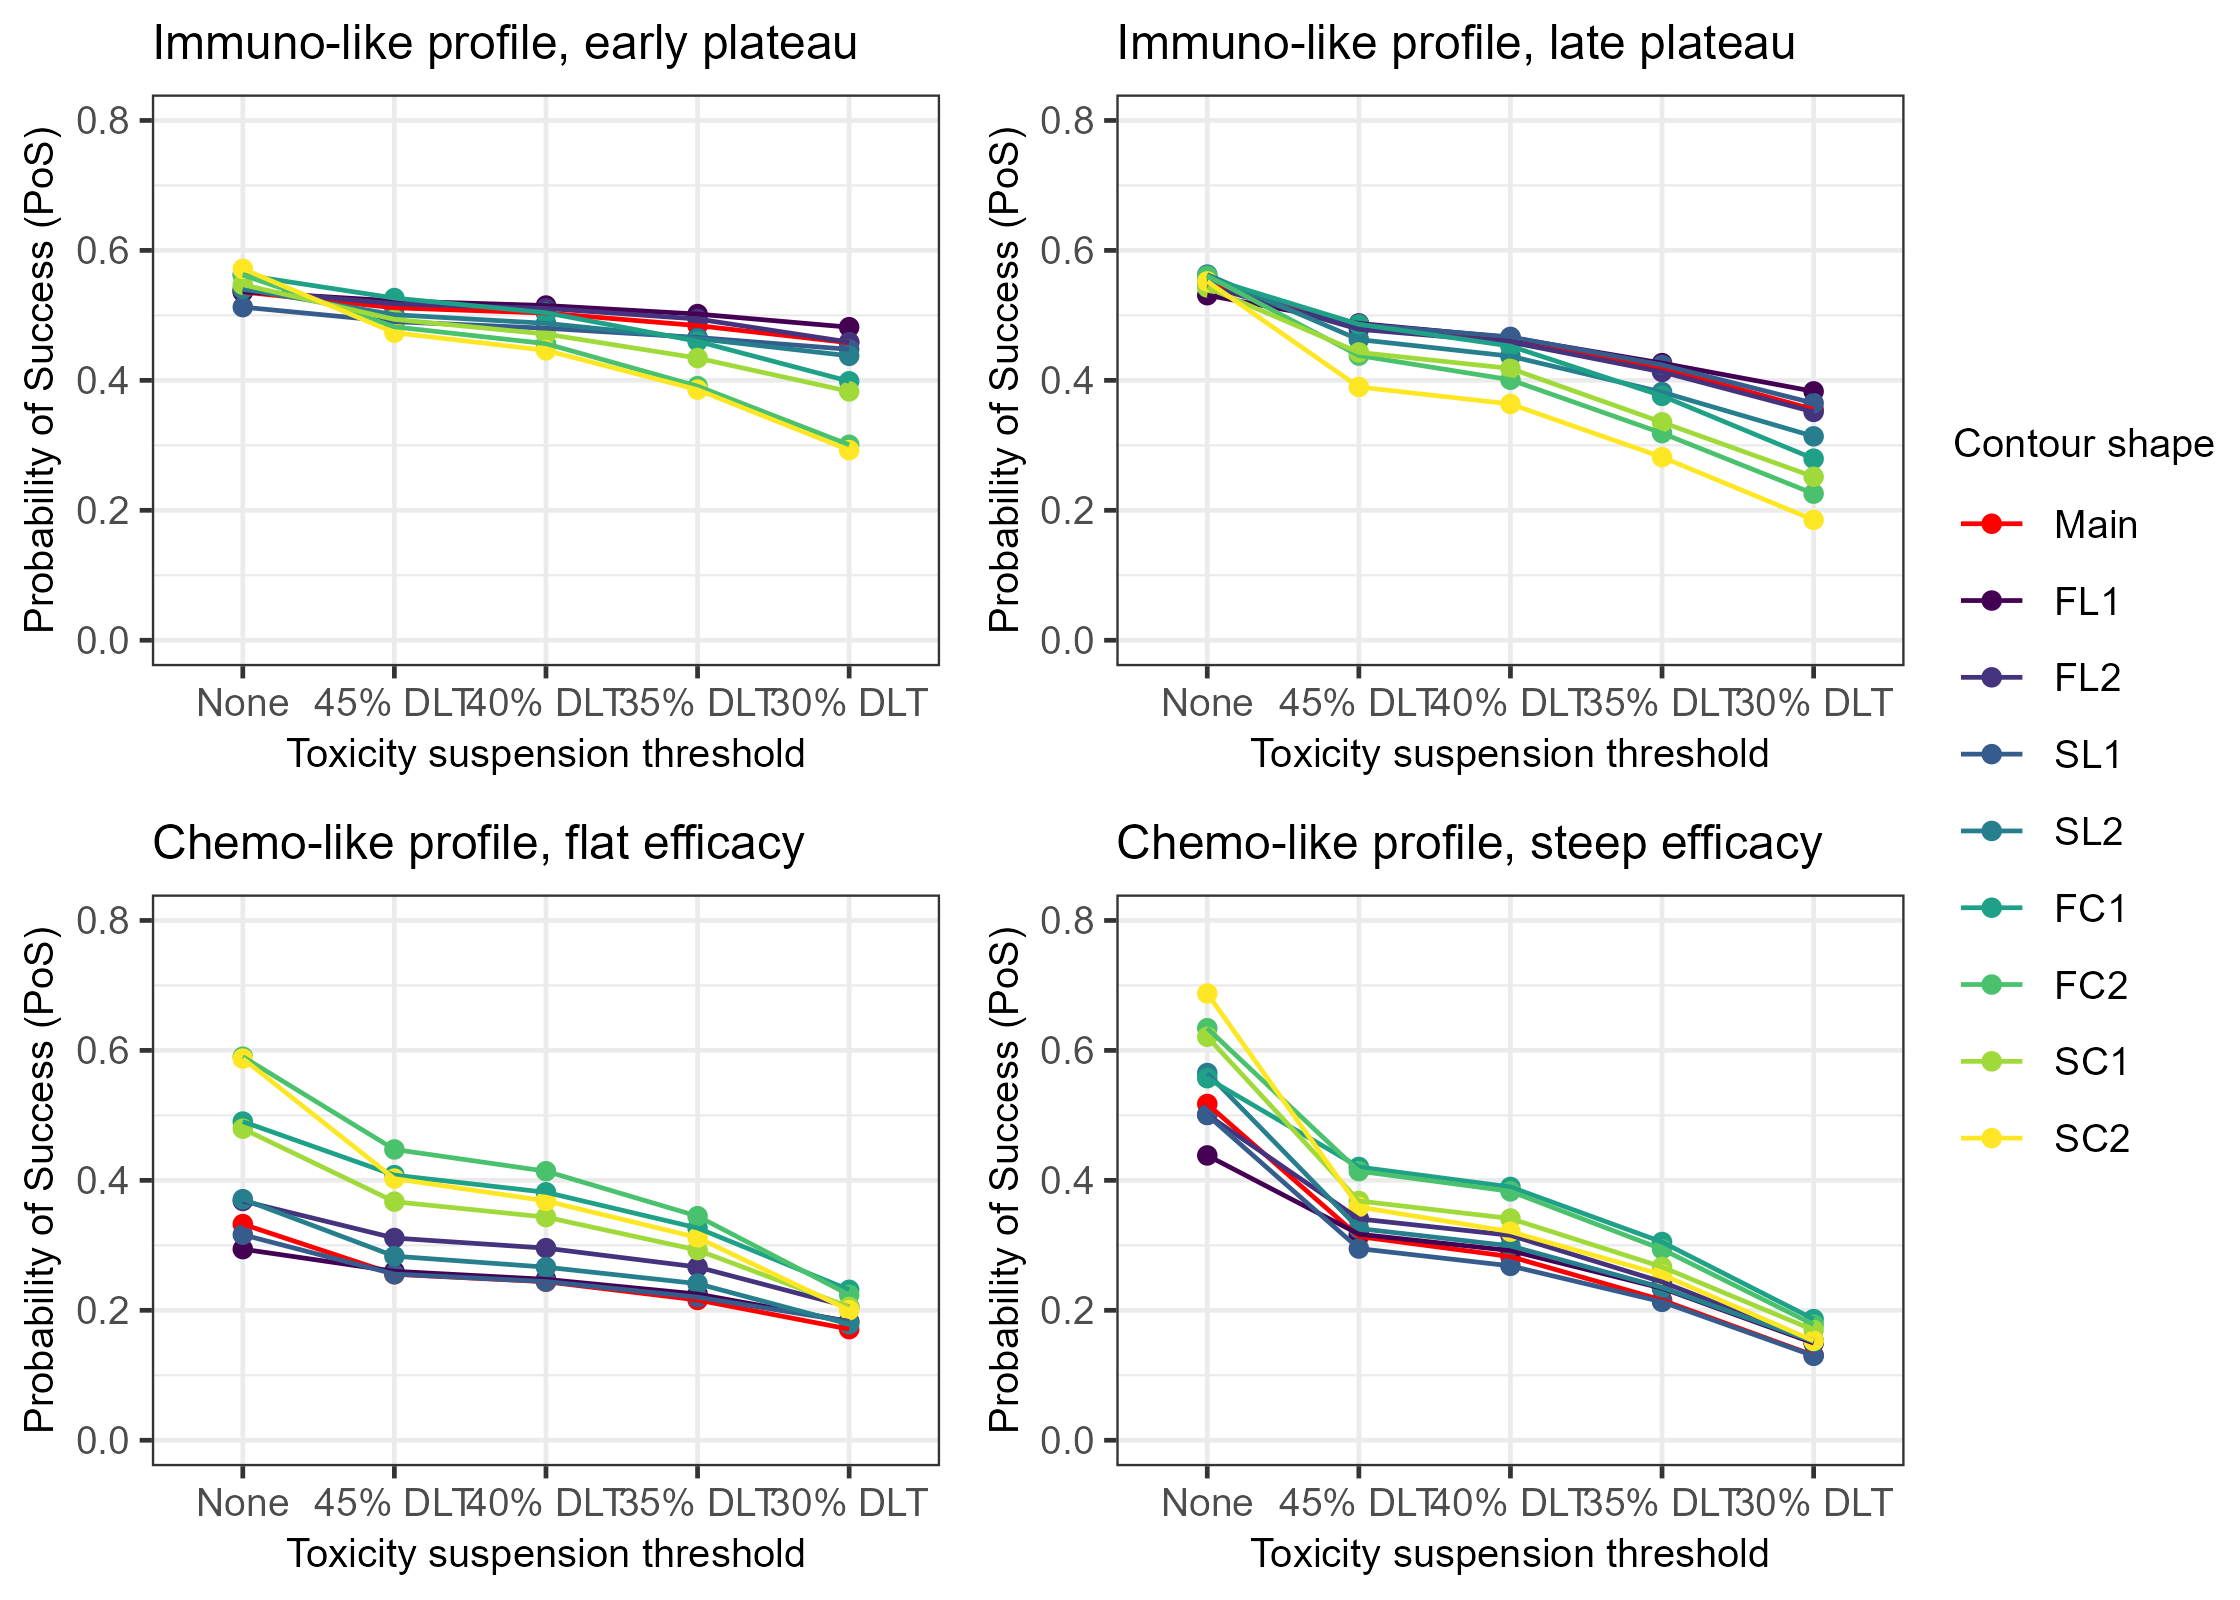
\includegraphics[width=0.9\textwidth]{plots/supplement/sens_EffTox_PoS.png}
    \caption{Probability of overall success (PoS) of EffTox across different contour specifications for chemotherapy-like and immunotherapy-like drug profiles. The red line represents the result from the main simulation.}
    \label{plot-sens-EffTox-PoS}
\end{figure}

\begin{figure}[htbp]
    \centering
    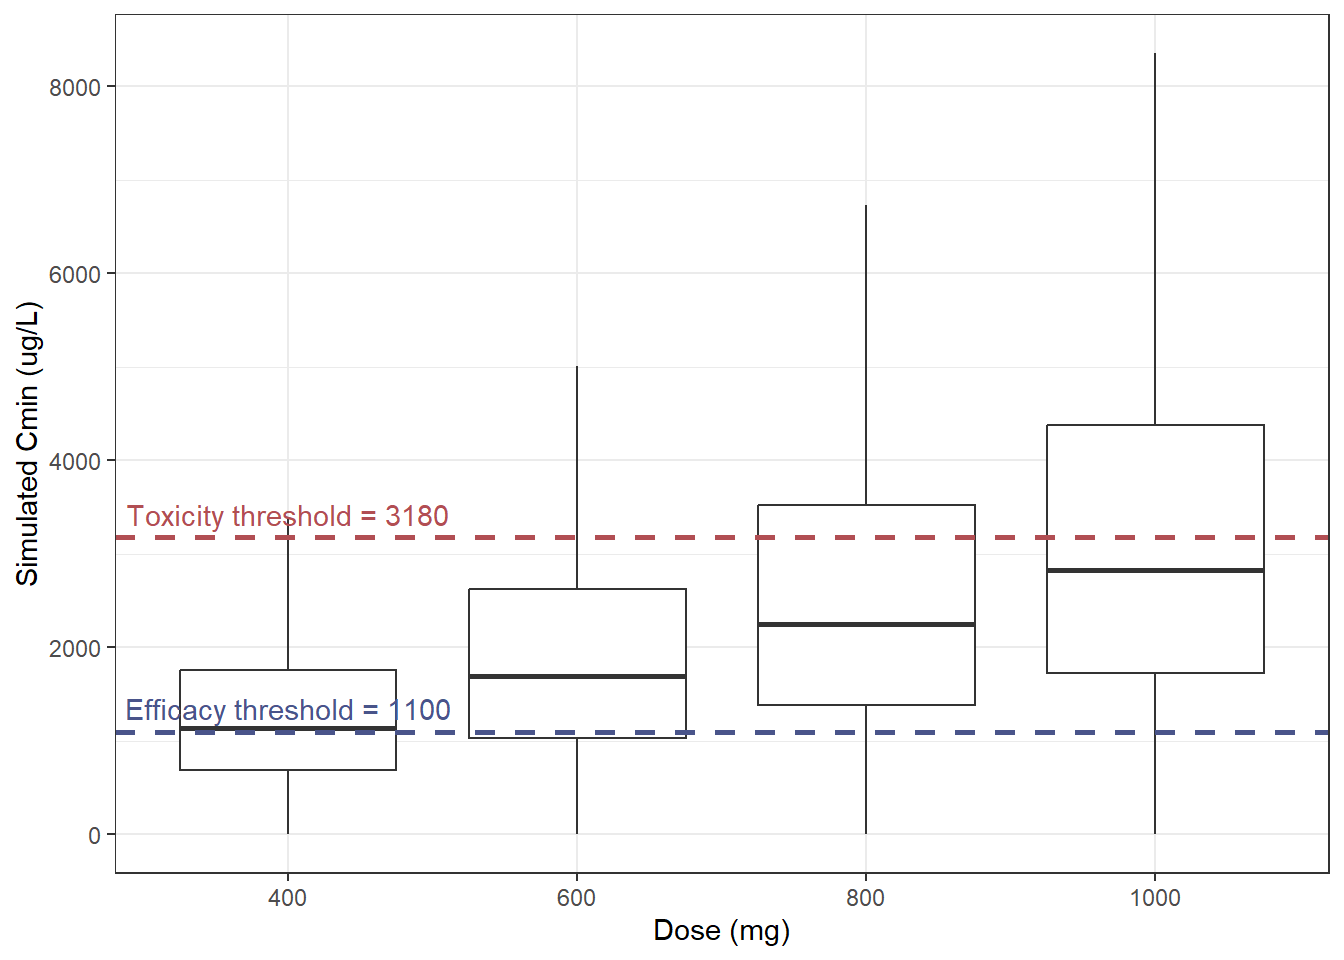
\includegraphics[width=0.9\textwidth]{plots/supplement/Dist_Imatinib_Cmin.png}
    \caption{Distribution of simulated Cmin values for Imatinib at doses of 400, 600, 800, and 1000 mg}
    \label{Dist-Imatinib-Cmin}
\end{figure}

\begin{figure}[htbp]
    \centering
    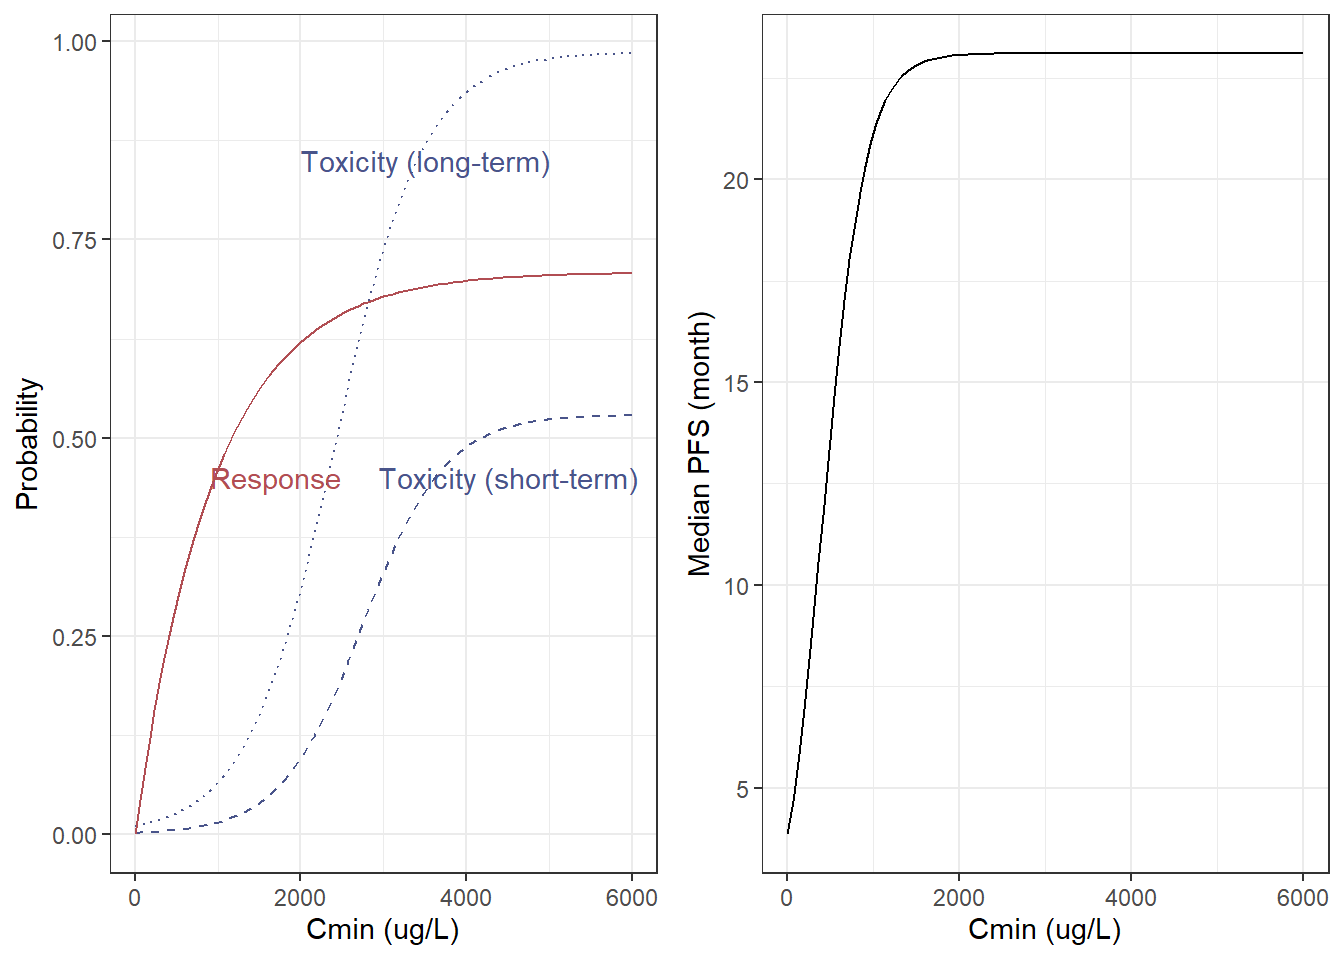
\includegraphics[width=0.9\textwidth]{plots/supplement/Imatinib_exposure_outcome.png}
    \caption{Exposure-toxicity (short/long-term), exposure-response, and exposure-PFS (progression-free survival) curves for Imatinib. }
    \label{Imatinib-exposure-outcome}
\end{figure}
\end{document}